\documentclass[review]{elsarticle}

\usepackage[colorlinks]{hyperref}
\usepackage[colorinlistoftodos]{todonotes}
\usepackage{verbatim}
\usepackage[utf8]{inputenc}
\usepackage[T1]{fontenc}
\usepackage{adjustbox}
\usepackage{multirow}
\usepackage{longtable}
\usepackage{booktabs}
\usepackage{lineno,hyperref}
\usepackage{listings}
\modulolinenumbers[5]

\journal{colleagues for review}

%%%%%%%%%%%%%%%%%%%%%%%
%% Elsevier bibliography styles
%%%%%%%%%%%%%%%%%%%%%%%
%% To change the style, put a % in front of the second line of the current style and
%% remove the % from the second line of the style you would like to use.
%%%%%%%%%%%%%%%%%%%%%%%

%% Numbered
%\bibliographystyle{model1-num-names}

%% Numbered without titles
%\bibliographystyle{model1a-num-names}

%% Harvard 
%\bibliographystyle{model2-names.bst}\biboptions{authoryear}

%% Vancouver numbered
%\usepackage{numcompress}\bibliographystyle{model3-num-names}

%% Vancouver name/year
%\usepackage{numcompress}\bibliographystyle{model4-names}\biboptions{authoryear}

%% APA style
\bibliographystyle{model5-names}\biboptions{authoryear}

%% AMA style
%\usepackage{numcompress}\bibliographystyle{model6-num-names}

%% `Elsevier LaTeX' style
%\bibliographystyle{elsarticle-num}
%%%%%%%%%%%%%%%%%%%%%%%

\begin{document}

\begin{frontmatter}

%% Title, authors and addresses

\title{Shape difference or shape change? Inter-regional variation in Gahagan biface morphology}

%% use the tnoteref command within \title for footnotes;
%% use the tnotetext command for the associated footnote;
%% use the fnref command within \author or \address for footnotes;
%% use the fntext command for the associated footnote;
%% use the corref command within \author for corresponding author footnotes;
%% use the cortext command for the associated footnote;
%% use the ead command for the email address,
%% and the form \ead[url] for the home page:
%%
%% \title{Title\tnoteref{label1}}
%% \tnotetext[label1]{}
%% \author{Name\corref{cor1}\fnref{label2}}
%% \ead{email address}
%% \ead[url]{home page}
%% \fntext[label2]{}
%% \cortext[cor1]{}
%% \address{Address\fnref{label3}}
%% \fntext[label3]{}


%% use optional labels to link authors explicitly to addresses:
%% \author[label1,label2]{<author name>}
%% \address[label1]{<address>}
%% \address[label2]{<address>}
%% Group authors per affiliation:
\author{Robert Z. Selden, Jr.\textsuperscript{a,b,c*}, John E. Dockall\textsuperscript{d,e}, and Morgane Dubied\textsuperscript{f}}
\address[1]{Heritage Research Center, Stephen F. Austin State University, United States}
\address[2]{Cultural Heritage Department, Jean Monnet University, France}
\address[3]{ORCID ID \href{http://orcid.org/0000-0002-1789-8449}{0000-0002-1789-8449}}
\address[4]{Prewitt and Associates, Inc., United States}
\address[5]{ORCID ID \href{http://orcid.org/0000-0002-0940-7144}{0000-0002-0940-7144}}
\address[6]{UMR 6282, Laboratoire Biogéosciences, Université de Bourgogne, France}
\cortext[cor1]{Corresponding author, Robert Z. Selden, Jr. (zselden@sfasu.edu)}

\begin{abstract}
This investigation aggregates intact or reconstructed Gahagan bifaces from the Caddo and central Texas regions to test the hypothesis that Gahagan biface morphology differs between them. The bifaces were scanned, then analysed using the tools of geometric morphometrics. Results provide a preview of those morphological differences that occur in Gahagan bifaces found at Caddo and central Texas sites. The size discrepancy represents an inversion of theoretical constructs that posit a decrease in tool size thought to articulate with an increase in distance from raw material source, as the Caddo sample is thought to have been produced primarily of Edwards chert from central Texas. One hypothesis (shape difference) posits that the contrasting morphologies represent two discrete communities of practice; one (central Texas hunter-gatherers) where the bifaces were utilised for practical purposes, and the other (Caddo horticulturalists) where Gahagan bifaces were enlisted primarily for burial and ritualistic activities. An alternative hypothesis (shape change) posits that Gahagan bifaces may have served multiple functions in Caddo society that differed in their deployment within and beyond the southern Caddo area.
\end{abstract}

\begin{keyword}
NAGPRA \sep 3D geometric morphometrics \sep museum studies \sep digital humanities \sep virtual archaeology
\end{keyword}

\end{frontmatter}

\linenumbers

\section*{}

\begin{quote}
The mathematical definition of a ``form'' has a quality of precision which was quite lacking in our earlier stage of mere description; it is expressed in few words, or in still briefer symbols, and these words or symbols are so pregnant with meaning that thought itself is economised \citep[720-721]{RN11532}.    
\end{quote}

This contribution follows a recent study of Gahagan biface morphology that enlisted the three largest samples from the Gahagan Mound (16RR1), George C. Davis (41CE19), and Mounds Plantation (16CD12) sites in the southern Caddo area (Figure ~\ref{fig:figmap}) \citep{RN11783}. The results of that study indicated a significant difference in shape for Gahagan bifaces found at the Mounds Plantation site when compared with those found at the Gahagan Mound and George C. Davis sites \citep[Figure 7]{RN11783}. The test for morphological disparity indicated that the sample from Gahagan Mound occupied a significantly greater range of morphospace than the sample from Mounds Plantation, providing limited evidence for discussions of specialisation and diversity. Morphological integration was also significant, meaning those traits used to characterise Gahagan biface shape (blade and base) were found to vary in a coordinated manner. The results confirmed the supposition advanced by \cite{RN3684} that the assemblage of Gahagan bifaces from the George C. Davis site compares favourably with those reported from the Gahagan Mound site \citep{RN5274,RN2740}.

\begin{figure}[ht]\centering
\includegraphics[width=\linewidth]{gahagan-map.pdf}
\caption{Site locations for collections used in the analysis. Southern Caddo area in white, and Brazos County (outlined in black) located to the southwest. The Doerge collection is from Brazos County, Texas, and the provenance of the BVMNH collection is unknown, but is assumed to be central Texas.}
\label{fig:figmap}
\end{figure}

The shape difference identified in the previous study occurs across the same geography as a difference in Smithport Plain and Hickory Engraved (Caddo) bottle shapes \citep{RN11801,RN11782,RN11716,RN20852}. The difference in Caddo bottle morphology has been attributed to two Formative/Early Caddo communities of practice---one north, and the other south---where the same decorative motifs were applied to two distinct vessel shapes. The shape boundary found to occur in Smithport Plain and Hickory Engraved bottles \citep[Figure 1]{RN20852} also manifests in Gahagan bifaces where the difference in shape was expressed spatially between the Gahagan Mound and Mounds Plantation sites \citep{RN11783}. 

The Gahagan type was suggested by Clarence H. Webb at the Caddo Conference in 1970 \citep{RN3684}, and was intended as a replacement for what \cite{RN800} had previously called Copena knives based upon similarities in form, but not---according to \cite{RN3684}---technology, between specimens found at the George C. Davis site and those reported by \cite{RN11562} in Alabama. Gahagan bifaces were named for the finely-crafted bifaces found by \cite{RN2740} at Gahagan Mound \citep{RN3684}. \citet[22]{RN4924} later advanced a description for the type, but a comparison of the technological attributes needed to gainfully discriminate between Gahagan and Copena bifaces was not provided. 

Additional specimens have been added to the sample used in the previous analysis from known Caddo sites (Doc Marks and Pelican), which are contrasted with those recovered from central Texas sites (Bastrop State Park and Doerge Collection), and one unprovenienced collection from the Brazos Valley Museum of Natural History (BVMNH) (Figures ~\ref{fig:figmap} and ~\ref{fig:fig2}), providing those data needed to test whether Gahagan biface morphology in central Texas differs from those found at Caddo sites in east Texas. The Doerge Collection is a large private collection that was donated to the BVMNH, and includes the largest collection of Gahagan bifaces found outside of the southern Caddo area \citep[Table 5]{RN4924}. No site-specific details were provided to the museum related to context, association, or cultural affiliation; however, the museum was informed that the whole of the collection was from Brazos County, Texas. Another small collection of Gahagan bifaces are curated at BVMNH, are unprovenienced, and assumed to come from the central Texas region. The single specimen from Bastrop State Park was found on the surface at the Rylander site (41BP882) by Emmy Lyn Francell, and is curated at the Texas Parks and Wildlife Department. There are no chronometric dates associated with any of the central Texas archaeological contexts used in this study.

\begin{figure}[htbp]\centering
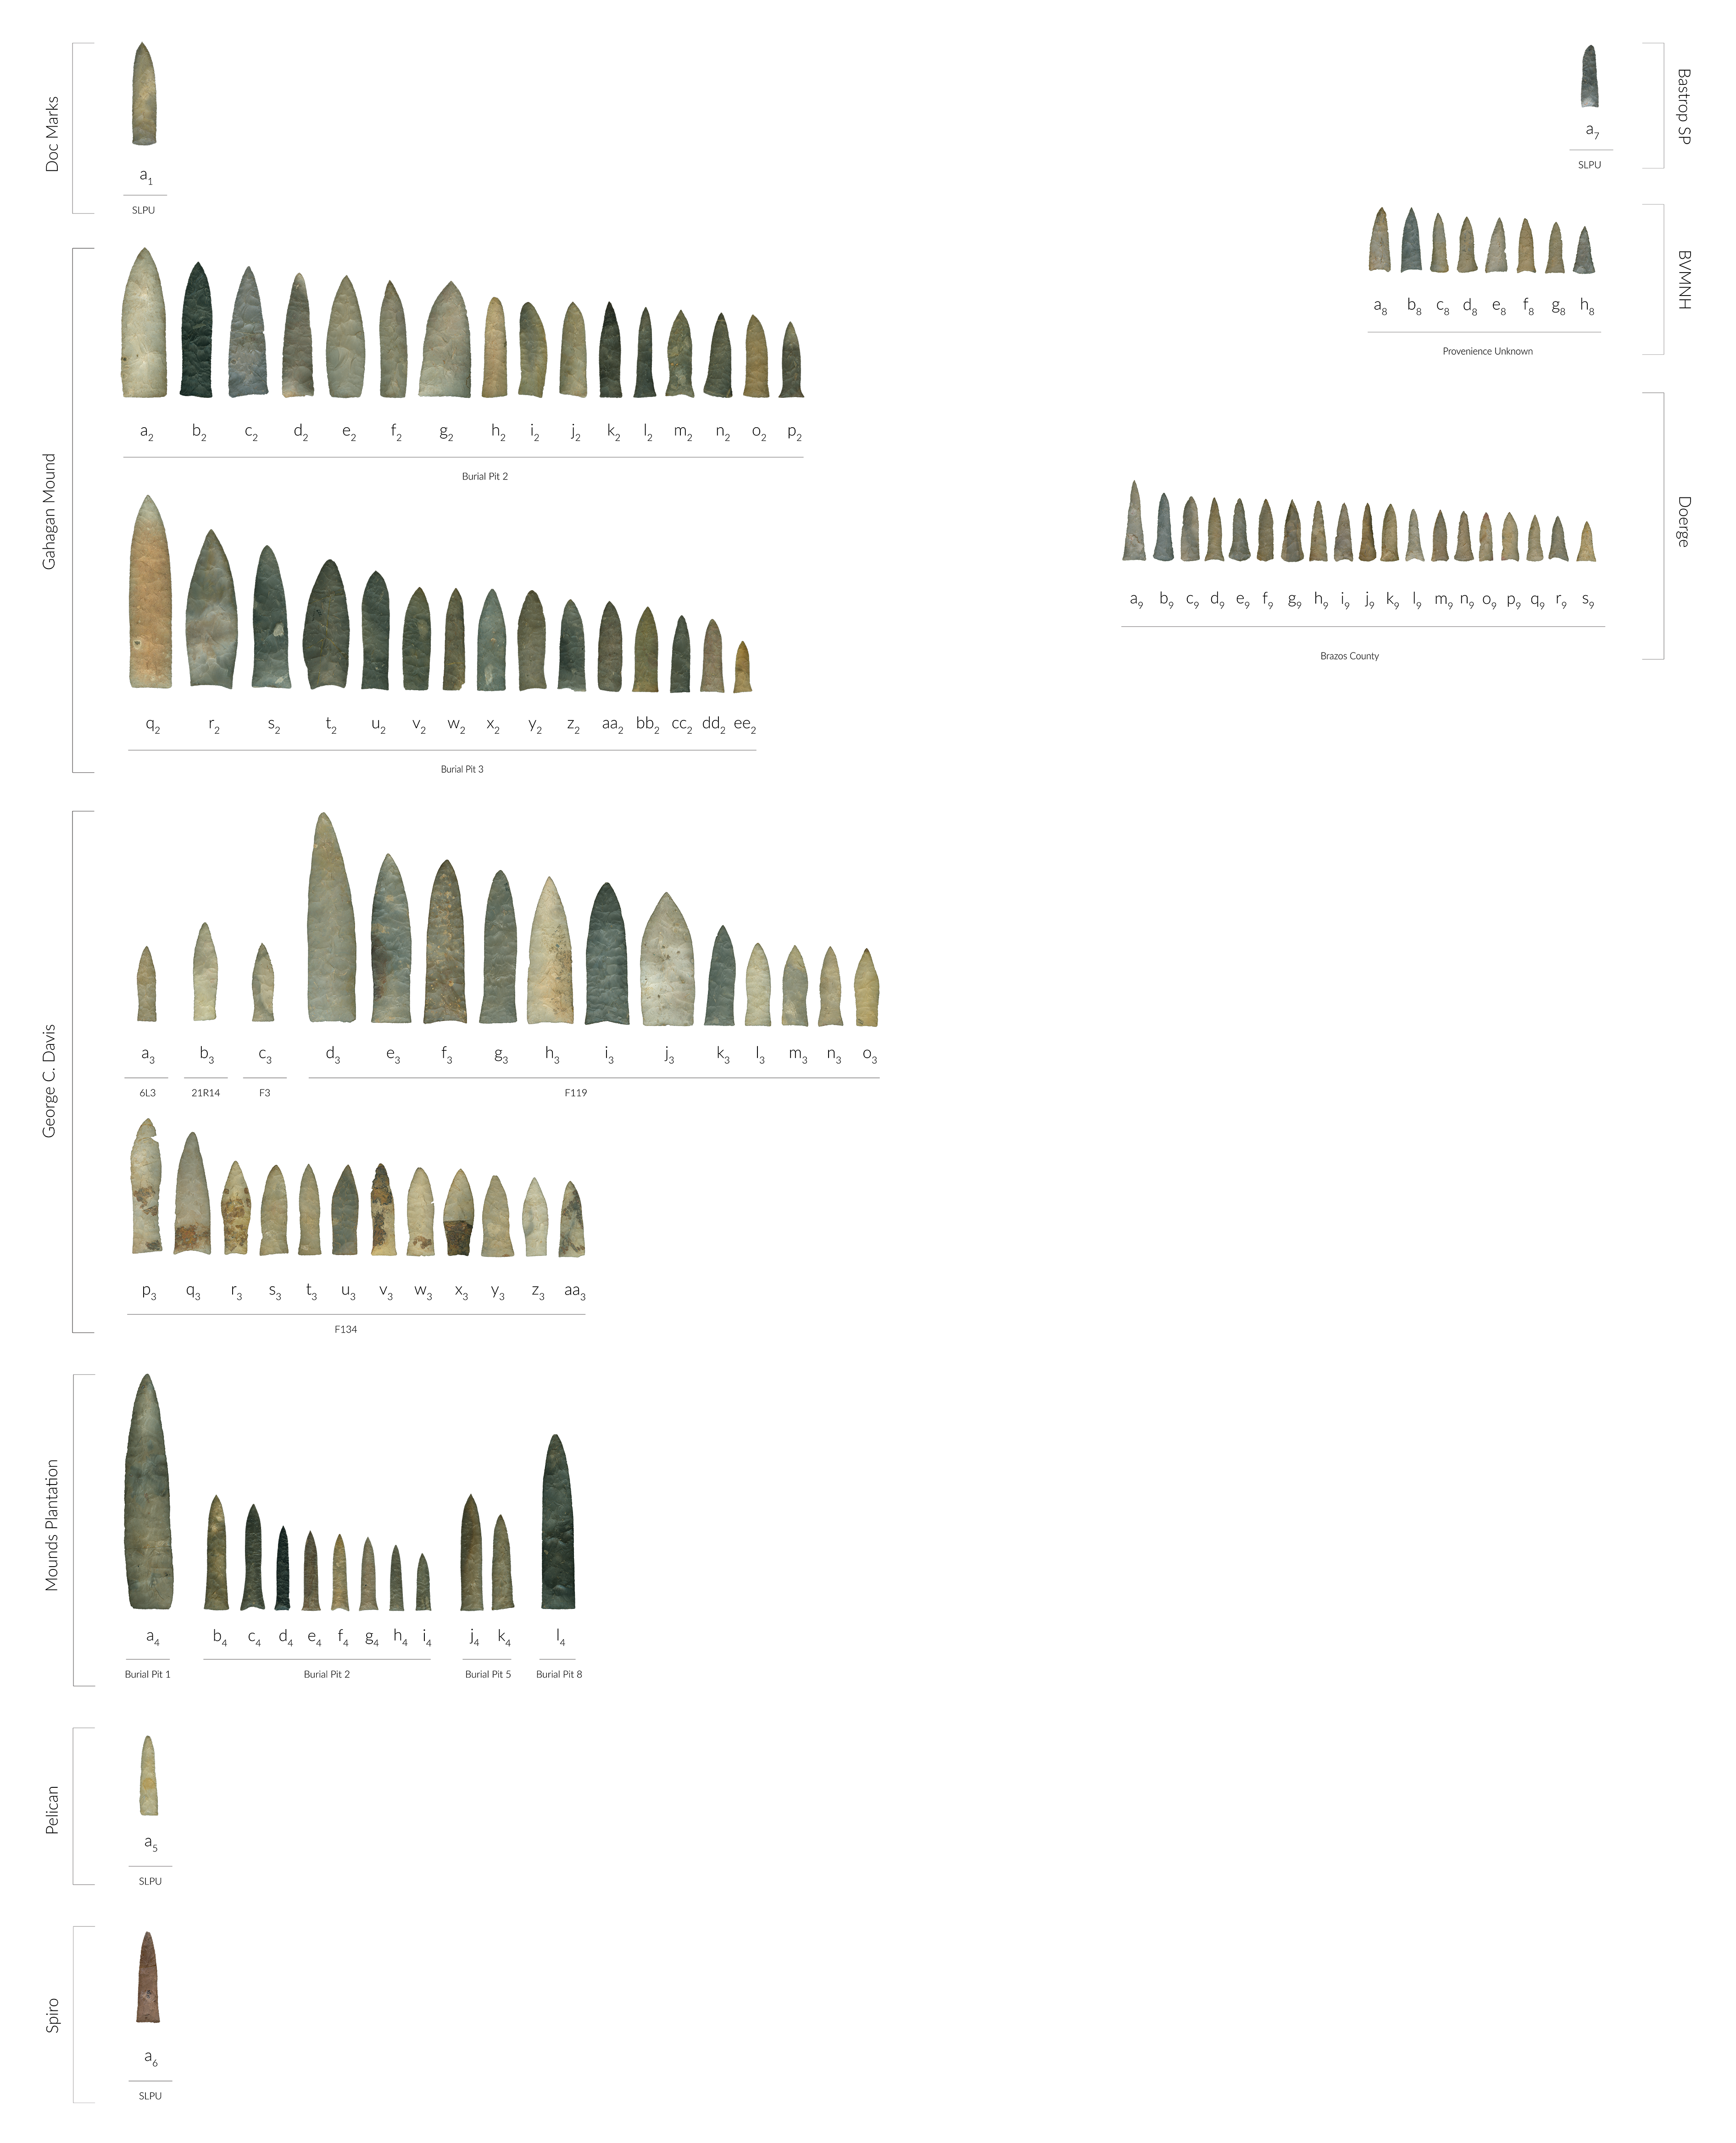
\includegraphics[width=\linewidth]{fig02}
\caption{Gahagan bifaces from known Caddo (left) and central Texas sites (right) organised by context and length; a1, no site-level provenience; a2, 569; b2, 543; c2, 551; d2, 541; e2, 546; f2, 544; g2, 545; h2, 489; i2, 532; j2, 548; k2, 550; l2, 533; m2, 549; n2, 547; o2, 490; p2, 542; q2, 593; r2, 666; s2, 605; t2, 622; u2, 606; v2, 609; w2, 623; x2, 608; y2, 607; z2, 662; aa2, 611; bb2, 610; cc2, 612; dd2, 613; ee2, 614; a3, ET221-993; b3, ET221-1260A; c3, ET221-1016; d3, 463-1; e3, 424-39; f3, 424-53; g3, 424-50; h3, 424-41; i3, 424-221; j3, 424-218; k3, 463-16; l3, 424-230; m3, 463-23; n3, 424-169; o3, 424-33; p3, 4078-8; q3, 4078-9; r3, 4078-11; s3, 4078-72; t3, 4078-45; u3, 4078-12; v3, 4078-13; w3, 4078-72; x3, 4078-14; y3, 4078-32; z3, 4078-22; aa3, 4078-14; a4, 3Ba90; b4, 3Bb6; c4, 3Bb1; d4, ThnBlk; e4, 3Bb7; f4, 3Bb3; g4, 3Bb4; h4, 3Bb8; i4, 3Bb5; j4, Case2LG; k4, Case2SM; l4, LGGray; a5, no site-level provenience; a6, no site-level provenience; a7 - h7, no provenience; a8 - s8, Brazos County, Texas. Bifaces w2, z2, and aa3 were not used in the analysis due to basal fractures, but are included here for visual comparative purposes. Additional information for each specimen, including the option to download the 2D images, can be found at \href{https://scholarworks.sfasu.edu/ita-gahaganbiface/}{https://scholarworks.sfasu.edu/ita-gahaganbiface/}.}
\label{fig:fig2}
\end{figure}

This effort expands upon the previous study through a comparison of Gahagan bifaces from the southern Caddo area, and the neighbouring central Texas region. Preliminary observations point to significant morphological differences between Gahagan bifaces recovered from Caddo and central Texas sites. Gahagan bifaces, a descriptive type including both morphological and chronological characteristics \citep{RN20847}, have long been leveraged as diagnostic markers of Formative and/or Early Caddo occupations \citep{RN4924,RN3684}. Should the morphology of Gahagan bifaces from central Texas be found to differ from those recovered from the southern Caddo area, additional theoretical explanations may be warranted. One possibility (shape difference) may be that two communities of practice existed for Gahagan bifaces. An alternative explanation (shape change) may be situational, demonstrating that Gahagan bifaces served multiple functions within Caddo society; one applied within the southern Caddo area, and another beyond.

\subsection*{Context}

The flexuous blade shapes associated with Gahagan bifaces from Burial 1 at the Gahagan Mound site led to the initial interpretation that they were knives \citep[Figures 18-21]{RN2740}. A subsequent investigation at the Gahagan Mound site \citep{RN5274} classified the bifaces into two different biface types (both currently designated as Gahagan bifaces); one made of dull gray chert with a square base and a symmetrical or curved knife form, and the other made of semi-translucent flint with a curved base and more strongly curved sides. In Burial Pit 2 at Gahagan Mound \citep[Plate 21]{RN5274}, one Gahagan biface (Figure ~\ref{fig:fig2}, a2) \citep[Plate 27, No. 1, 3]{RN5274} was found near the left shoulder of an adult male (Skeleton 3), but most artefacts were recovered near the northwest margin of the burial pit, including the remaining Gahagan bifaces associated with that context. In Burial Pit 3 at Gahagan Mound \citep[Plate 23, 1]{RN5274}, one Gahagan biface was found near the left femur of Skeleton 1 (Figure ~\ref{fig:fig2}, r2) \citep[Plate 27, No. 1, 2]{RN5274}. Similar to Burial Pit 2, most of the artefacts from Burial Pit 3 were found along the northwest margin, including the remainder of Gahagan bifaces from that context \citep{RN5274}.

At the George C. Davis site, two Gahagan bifaces were found outside of mound or feature contexts (Figure ~\ref{fig:fig2}, a3 and b3), and their feature assignments (6L3 and 21R14) articulate with the excavation grid used by \cite{RN800}. Feature 3 is associated with a 27-foot diameter ring of 35 postholes located east of Mound A \citep[Figure 4]{RN800}, where one Gahagan biface (Figure ~\ref{fig:fig2}, c3) was found in the outlining postholes \cite{RN800}.

Feature 134 is associated with a Stage I burial feature at the George C. Davis site that predates the construction of Mound C, and contained eight individuals \citep{RN808,RN5050}. One large (48 cm), well-thinned biface that \citet[22]{RN808} listed as a “Gahagan?” biface was found near the right leg of Skeleton 5.  \citet[Figure 19x]{RN3684} included this specimen---and one additional large specimen from Feature 119 \citep[Figure 19w]{RN3684}---in his Group 2 bifaces due to a lack of the fine pressure-flaked margins definitive of Group 1 (Gahagan) bifaces. Nine Gahagan bifaces from Feature 134 were recovered from Concentration 2; seven (Figure ~\ref{fig:fig2}, p3-r3, u3, v3, x3, and aa3) were found “about and under gray pigment,” and two others were found outside of the pigmented area (Figure ~\ref{fig:fig2}, s3, w3) \citep[21-23 and Figure 12]{RN808}. Organic residue can still be found on a selection of these Gahagan bifaces \citep[Figure 2]{RN11783}, which \citet[228]{RN3684} notes, “may be the remains of leather or bark sheaths or cane wrapping.” Three additional Gahagan bifaces (Figure ~\ref{fig:fig2}, t3, y3, and z3) were found in Concentration 3 \citep[21-22 and Figure 12]{RN808}.

Feature 119 \citep[Figure 13-18]{RN808} articulates with a Stage II burial feature at the George C. Davis site that can be traced from the surface of the second mound stage, and included offerings associated with two discrete layers \citep{RN808,RN5050,RN806}. The first layer offerings include Gahagan bifaces from Concentration 1 (Figure ~\ref{fig:fig2}, o3), Concentration 2 (Figure ~\ref{fig:fig2}, e3, g3, h3, and n3), and Concentration 3 (Figure ~\ref{fig:fig2}, f3, i3, j3, and l3). Second layer offerings include Gahagan bifaces associated with Concentration 1 (Figure ~\ref{fig:fig2}, d3), Concentration 3 (Figure ~\ref{fig:fig2}, m3), and Skeleton 1 (Figure ~\ref{fig:fig2}, k3). 

Burial Pit 2 at Mounds Plantation is the only context that contained a single individual, and \citet[97]{RN11561} noted that “fine edge retouch leaves the edges with almost no serration or irregularity, altogether the finest flint knapping that we have seen from a Caddoan site” (Figure ~\ref{fig:fig2}, b4-i4). The bifaces from Burial Pit 2 at Mounds Plantation were found in a bundle, but those from Burial Pit 5 articulate with the males of Groups 1 and 2 (Figure ~\ref{fig:fig2}, j4 and k4, respectively), and were found in a context parallel to the left forearm, pointed toward the hand \citep[Figure 5]{RN11561}. The biface from Burial Pit 8 at Mounds Plantation (Figure ~\ref{fig:fig2}, l4) was found in the same position on the left forearm; however, the largest biface (Burial Pit 1, Skeleton 1; see Figure ~\ref{fig:fig2}, a4) was found across the chest of that individual \citep{RN11561}.

McKinney posited that Gahagan bifaces may have been carried in a sheath attached to the left forearm \citep{RN11561}. Similarly, \citet{RN3684} noted that---at the George C. Davis site---edge modification was confined to traces of polish and smoothing along the widest blade segments and near the tip on burial specimens, was more pronounced on specimens from non-mound contexts, and possibly represented sheath wear. The polish that \citet{RN3684} discussed supports McKinney’s hypothesis \citep{RN11561}, where the tip and lateral edges of the biface may have become polished while being worn in a sheath on the left forearm with the tip pointed toward the hand.

\subsection*{Chronometric dating}

\citet[Table 1]{RN4783} reported three AMS radiocarbon dates from Burial Pit 2 at the Gahagan Mound site. The first (UGA12296), from Deposit 3 in Burial Pit 2, was fragmented wood—possibly cypress—from a copper-covered wooden object that \citet[99, Plate 29, No. 2, Object 5]{RN5274} describe as a pendant in the shape of an animal claw \citep{RN4783}. The second (ISGS A0465), found adjacent to the head of Skeleton 3 (adult female) in Burial Pit 2, was unidentifiable fragmented wood that \citet[96, Plate 21 and 28, Nos. 2-3]{RN5274} describe as square ear ornaments of copper-coated cypress wood \citep{RN4783}. The third (ISGS A0466), from Deposit 2 in Burial Pit 2, was not described by \citet[96]{RN5274}, but \citet[62]{RN4783} describe it as a leather-covered copper object.

\citet[Table 1]{RN3714} reported two radiocarbon dates (Tx-913 and Tx-1206) from contexts associated with the special mortuary in Mound C at the George C. Davis site where Gahagan bifaces were found \citep[Table 5]{RN3714}. The date from Feature 119 (Tx-913) is associated with the green fill placed atop the Caddo remains in the Stage II burial in Mound C \citep{RN3714}. The date from Feature 134 (Tx-1206) provided an age that \citet{RN3714} believed to be inconsistent with the stratigraphic position of the sample, thus it is excluded from the chronological model. Neither of the legacy dates from the George C. Davis site account for isotopic fractionation.

\citet[72]{RN11561} reported three dates from two logs found in Burial Pit 5 at the Mounds Plantation site. Two of those (Tx-55 and M-1446), both from Log 1, were described by \citet[72]{RN11561} as coming “from the upper set of timbers, about 50 cm above the pit floor.” The third (Tx-56), from Log 6, was described by \citet[72]{RN11561} as coming from “Log 6…nearer the center of the pit and just above the pit floor.” None of these three legacy dates account for isotopic fractionation. \citet{RN11561} omit the Log 6 (Tx-56) date from further discussions of the site, thus it is omitted from the chronological model. None of the legacy dates from the Mounds Plantation site account for isotopic fractionation.

Six of the chronometric dates listed above were included in the chronological model for Caddo contexts where Gahagan bifaces have been found (Figure 3). The oxcAAR library (\href{https://github.com/ISAAKiel/oxcAAR}{https://github.com/ISAAKiel/oxcAAR}) was used to build the chronological model in R, which was executed using OxCal 4.3.2 \citep{RN5514,RN20716} and the IntCal13 calibration curve \citep{RN4406}. The chronological model demonstrates the modeled age range for contexts where a selection of those Gahagan bifaces used in this study were recovered \citep{RN20850}. All contexts were plotted as a single phase associated with the Gahagan biface type, and the two dates associated with Log 1 at Mounds Plantation (Tx-55 and M-1446) were combined using the R\_Combine function \citep{RN20850}. Sensitivity analyses demonstrated that agreement with the date from F119 at George C. Davis shifted only one or two percentage points in either direction throughout ten variable iterations, indicating that the model is stable.

\begin{figure}[ht]\centering
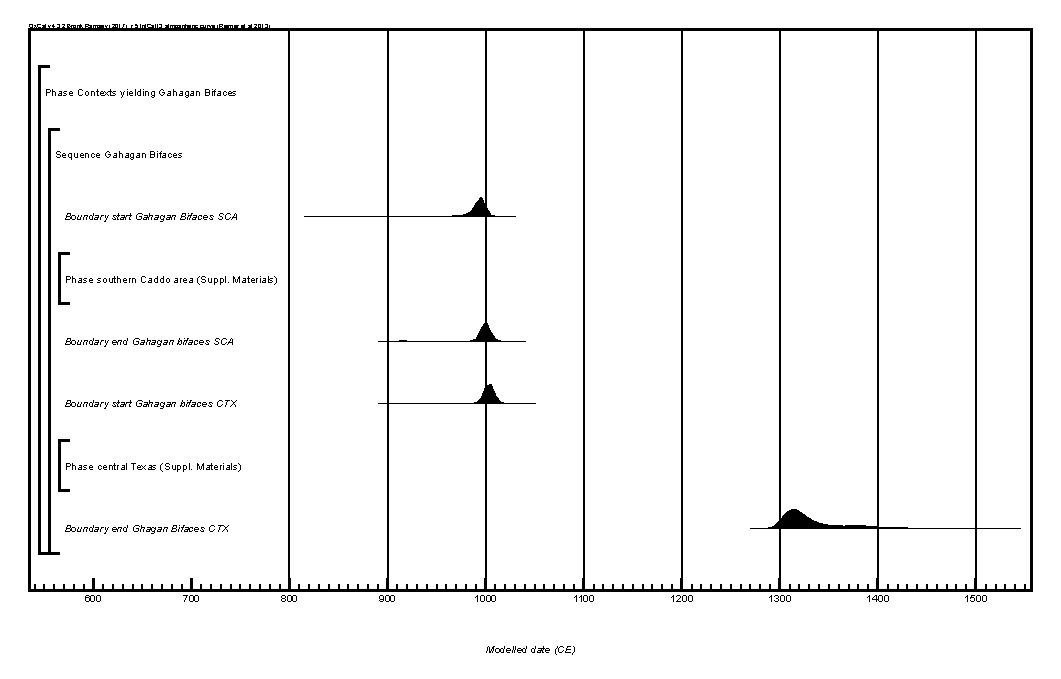
\includegraphics[width=\linewidth]{fig03}
\caption{Probability distributions for dates from contexts associated with Gahagan bifaces used in this study. Two distributions were plotted for each date or combination of dates; one represented by an outline that is the result of simple radiocarbon calibration, and the other in solid black, which articulates with the chronological model. The large square brackets down the left side of the diagram and the OxCal keywords define the model exactly. The oxcAAR script used to generate this figure is available in the supplementary materials at \href{https://github.com/aksel-blaise/gahaganmorph2/blob/master/analysis/gahagan14c.md}{https://github.com/aksel-blaise/gahaganmorph2/blob/master/analysis/gahagan14c.md}.}
\label{fig:fig3}
\end{figure}

\subsection*{Manufacture}

\citet{RN3684} discerned that all raw materials used in the manufacture of Gahagan bifaces found at the George C. Davis site were from non-local sources, which was a noteworthy revision to the initial interpretation by \citet{RN800}, in which the raw materials were considered to be of local origin. Further support for Shafer’s assertion is added in his discussion of the fragility of specimens coupled with the absence of failures in the extensive excavations at George C. Davis \citep{RN3684}. This observation aligns with findings from other locations \citep{RN1001}, where investigators demonstrated that Gahagan bifaces were manufactured with Woodford, Battiest, and Ogallala cherts, as well as cherts from the Kiamichi Mountains. \citet{RN3684} also noted the size and shape of Gahagan bifaces from the Davis site to be more uniform in Feature 134 compared with those from Feature 119, and that differences in the size of Gahagan bifaces from non-burial contexts were more striking than differences in shape.

\citet{RN3684} provides evidence for the presence of use-wear and fracture patterns on specimens from non-mound contexts at George C. Davis, suggesting that Gahagan bifaces from Caddo contexts may have functioned similarly to those used by hunter-gatherer groups. The occurrence of Gahagan bifaces in mound/burial and non-mound contexts at George C. Davis potentially indicates that they had secular and prestige/identity functions for Caddo peoples. In the analysis of debitage from George C. Davis, \citet{RN3684} argued that limited biface manufacture occurred at the site, but none of that debitage is directly attributable to Gahagan biface manufacture.

In addition to those Gahagan bifaces found at mound sites in the southern Caddo area, there is abundant evidence that similar bifaces were manufactured by contemporary hunter-gatherer groups in central and east-central Texas. Sites with evidence of manufacture and use can be found across a series of locations that fringe the eastern edge of the Balcones Escarpment \citep[Figure 5-3]{RN11568}. Each site is geographically situated on or within a zone of high-quality nodule and ledge cherts that may have served as source material. Gahagan bifaces found at these sites are represented by complete and incomplete specimens in varying stages of manufacture, use, maintenance, and discard. This indicates that bifaces were a commonly employed part of the overall lithic technology of central and east central Texas aboriginal groups, and likely used to perform a variety of common tasks.

A recent study tested the hypothesis that the manufacture of flat, thin bifaces—like Gahagan bifaces—would have yielded flatter bifacial thinning flakes that express low flake curvature \citep{RN11568}. The goal of that undertaking was to identify whether the flakes were distinctive enough on their own to warrant the assignment of potential Gahagan biface production locales, providing evidence for association of those production locales with the Prairie Caddo model \citep{RN4924} in the absence of diagnostic artefacts \citep{RN11568}. The results of that study demonstrated that bifacial thinning flake curvature was not sufficient as a marker of Gahagan biface production locales \citep{RN11568}.

In contrast to the Gahagan Mound, George C. Davis, and Mounds Plantation samples, there are currently no recorded instances of Gahagan bifaces from contexts in central Texas that might be interpreted as mortuary, religious, or ceremonial. Whether or not these bifaces served to denote individual status among hunter-gatherer groups is unknown, but they may have functioned as such during contact, exchange, or interaction between hunter-gatherers and Caddo groups to the east.

Production evidence is present at contemporary sites distributed on the eastern edge of the Balcones Escarpment. Sites like Urbankte (41CV26) and Penny Winkle (41BL22 and 41BL23), Iron Bridge (41BL47), Hoxie Bridge (41WM130), McDonald (41HI105), Loeve-Fox (41WM230), Grimes Houey (41CV17), J.B. White (41MM341) and locations on Fort Hood, have all yielded specimens representing manufacture, use and discard \citep{RN20717,RN11565,RN2708,RN20718,RN4924,RN20719}. Shafer posited that these bifaces were manufactured through a mix of hard and soft hammer percussion, as well as indirect percussion using a punch \citep{RN4924,RN3684}. Flake scar patterns on many Gahagan bifaces support the inference that indirect percussion was used as a shaping and thinning technique. Isolated finds across Bell, Williamson, Milam, McLennan, and other counties in central Texas suggest that Gahagan bifaces were manufactured and used in these areas \citep{RN4924}.

\subsection*{Analytical framework}

This basic research endeavour \citep{RN20851} consists of an exploratory analysis (Figure ~\ref{fig:exan}), and enlists the tools of geometric morphometrics to test whether Gahagan biface shape, size, and form differs between two archaeological regions. Landmark-based geometric morphometric methods are ideal for research designs that incorporate questions of complex 3D geometry. Examples from the literature cover a broad scope of artefact categories including projectile points \citep{RN1750,RN1755}, bifaces \citep{RN1727,RN4392,RN11550,RN11783}, percussive tools \citep{RN1772}, flake scars \citep{RN253}, flake tools \citep{RN11552}, handaxes \citep{RN1730,RN1766,RN3145,RN1733,RN335}, and Caddo ceramics \citep{RN1994,RN11521,RN11782,RN11801,RN11716,RN20852}. 

\begin{figure}[ht]\centering
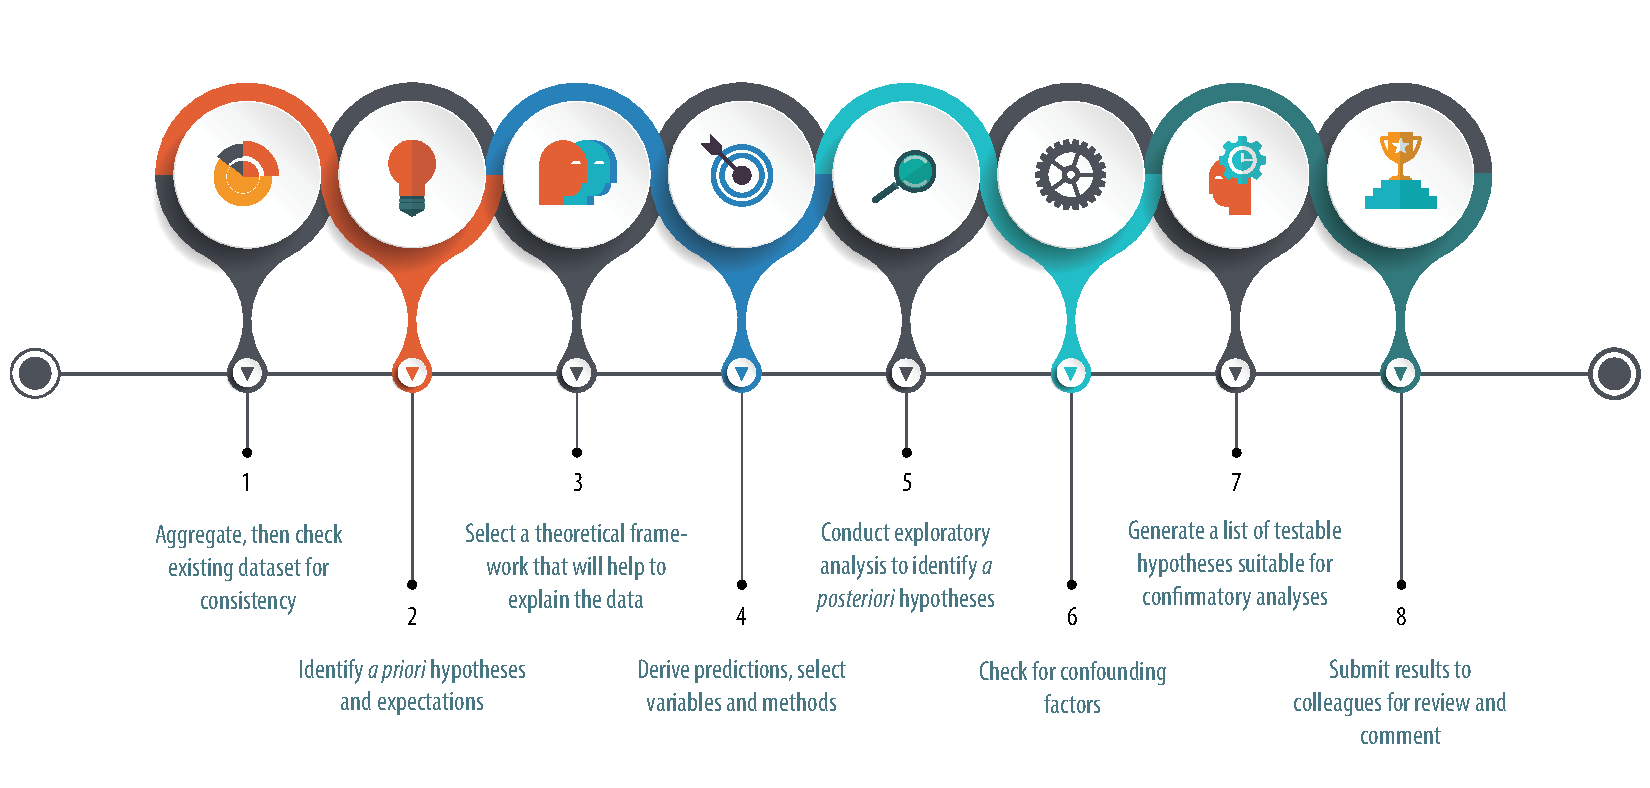
\includegraphics[width=\linewidth]{figexan.pdf}
\caption{Exploratory analysis workflow used in this study.}
\label{fig:exan}
\end{figure}

Analyses of artefact shape are neither new or novel \citep{RN11779}, and it is not surprising that geometric morphometrics (sensu \citet{RN11559}) has captivated analysts of material culture due to the substantive contribution of morphology to both ceramic \citep{RN1752,RN11631,RN4335} and lithic typologies \citep{RN11529,RN11528,RN20853,RN11534}, as well as additional categories of material culture \citep{RN1737,RN4374,RN11527}, and novel applications \citep{RN11543,RN11544}. Applications of GM in archaeology began with an analysis of irregular shapes by elliptic Fourier analysis (EFA) \citep{RN4379}, and iterative methodological improvements continue to expand the potential for analyses of shape as it relates to material culture (Figure ~\ref{fig:network}).

\begin{figure}[ht]\centering
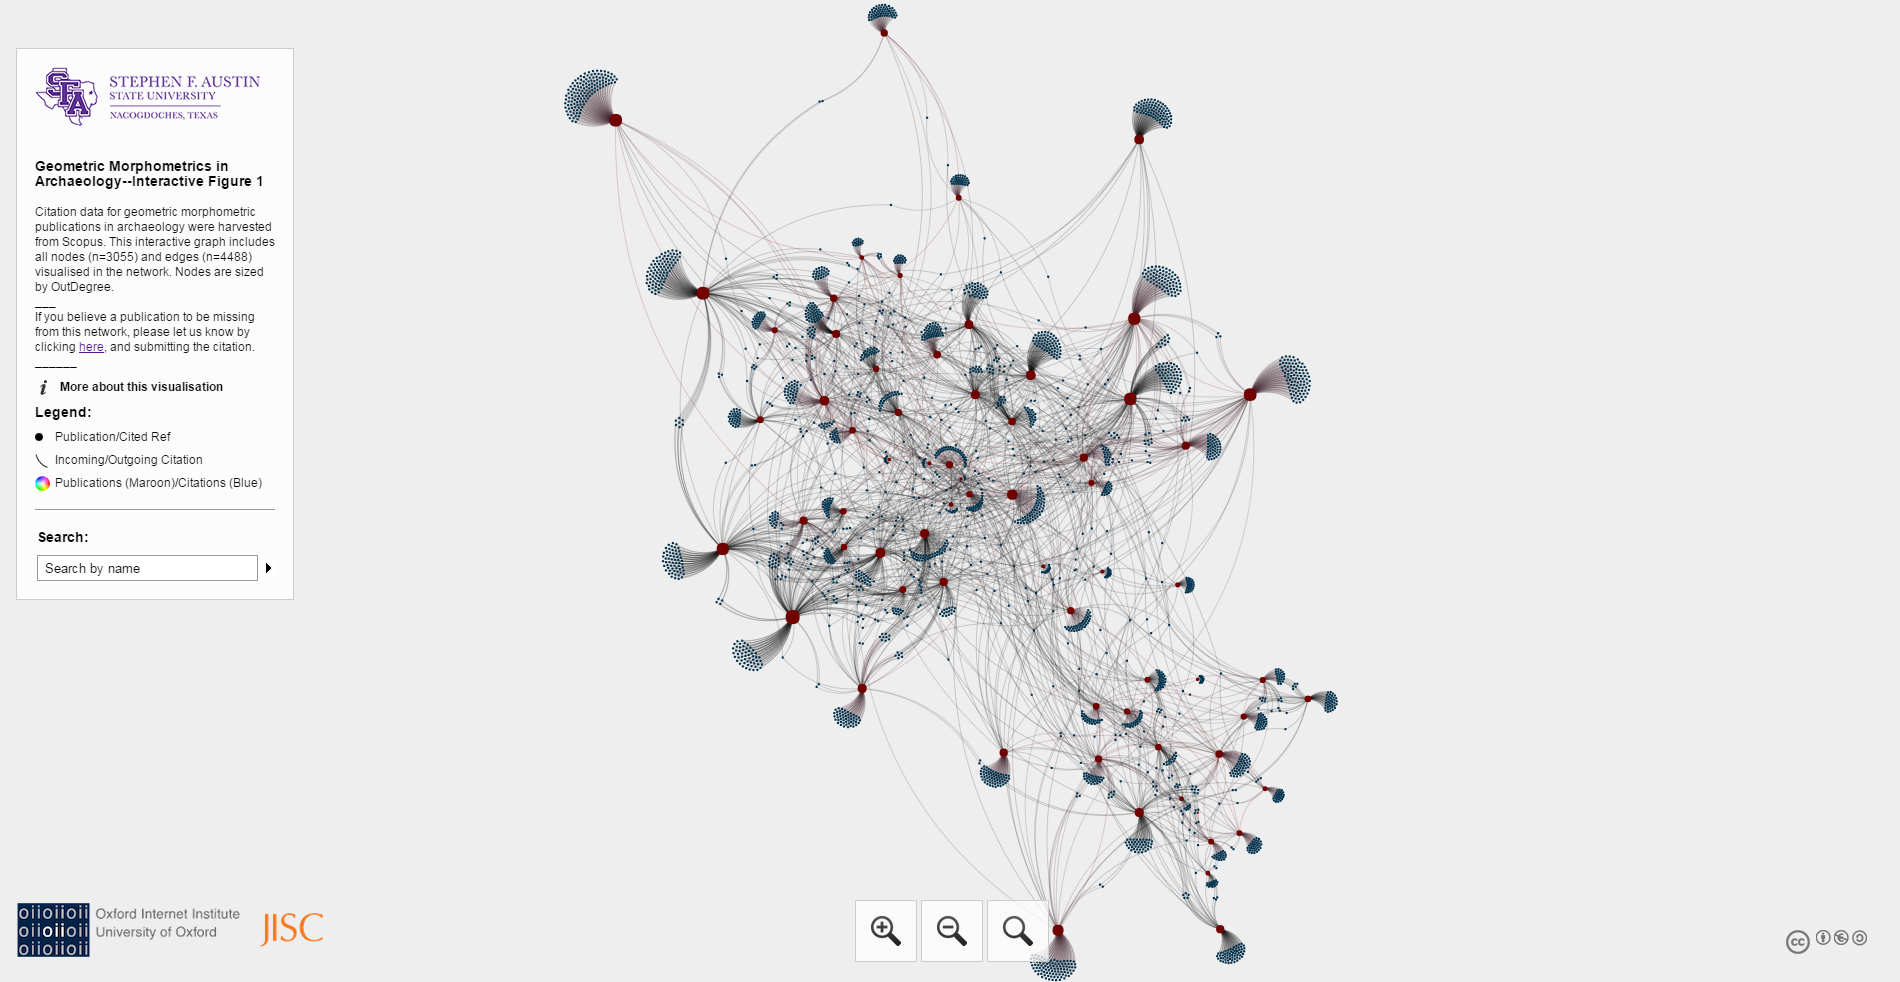
\includegraphics[width=\linewidth]{fignet.png}
\caption{Interactive citation network for geometric morphometric studies in archaeology, accessible at \href{http://crhr-archive.sfasu.edu/GMArchFig1/}{http://crhr-archive.sfasu.edu/GMArchFig1/}.}
\label{fig:network}
\end{figure}

The series of geometric morphometric studies focused upon Caddo ceramics has capitalised on the morphological variation that occurs along a single plane; however, 3D data were required to identify the widest vessel profile. The Gahagan bifaces used in the previous study come from many of the same contexts as the Caddo bottles, and were found to differ in morphology across the same shape boundary \citep[Figure 15.1]{RN11783,RN20852}. The current study takes advantage of a suite of analytical tools that have allowed for the incorporation of morphological attributes associated with beveling, which occurs with some regularity along the lateral edges of Gahagan bifaces.

\section*{Methods}

Each of the Gahagan bifaces was scanned with a Creaform GoSCAN 20 at a 0.3 mm resolution in VXelements. Scanner calibration was optimised prior to each scan with positioning targets required for increased accuracy and shutter speed reconfigured in each instance. A clipping plane was established to reduce the amount of superfluous data collected. Following data collection, the resolution of each mesh was increased to 0.1 mm, and the point cloud was transferred to VXmodel where the mesh was rendered following application of the \textit{clean mesh} function, used to remove isolated patches, self-intersections, spikes, small holes, singular vertices, creased edges, narrow triangles, outcropping triangles, narrow bridges, and non-manifold triangles prior to decimation and export as ASCII stl and ASCII ply. The stl functions as a 3D print-ready backup of the scan data, and the ply file was subsequently processed using the \textit{Rvcg} library in R 3.6.1 \citep{RN20849,R,RN20850} (Figure ~\ref{fig:figflow}).

\begin{figure}[ht!]\centering
\includegraphics[width=\linewidth]{gahagan-flow.png}
\caption{Workflow for data preparation used in this study. The pseudolandmarks generated by the \textit{auto3dgm} algorithm were employed as an exploratory tool, and were not used in the final analysis.}
\label{fig:figflow}
\end{figure}

There is a residue adhering to seven Gahagan bifaces from the George C. Davis site at variable thickness \citep[Figure 2]{RN11783}. \citet[228]{RN3684} posits that this residue potentially represents the remains of a sheath. While an interesting aside, the residue does pose a problem for an analysis of 3D geometry. The initial research design (3D) was thus revisited, leading to a reconfiguration of the previous analysis as a 2D geometric morphometric study \citep{RN11783}, enlisting a landmark configuration similar to that used by \citet[Figure 2]{RN1754}, \citet[Figure 2]{RN1736}, and \citet[Figure 1]{RN11731}. The residue does not occur on all of the George C. Davis specimens, and none of the Gahagan bifaces from the Mounds Plantation or Gahagan Mound sites include a similar residue on their surfaces, making it possible to compare a greater range of surface morphology between those samples. 

The same basic constellation of landmarks was employed for this undertaking; however, unlike the previous iteration where landmarks were populated along a spline, landmarks in this iteration were plotted directly on the 3D meshes, providing a means of capitalising on shape variation introduced through beveling. This configuration of landmarks will be revised in subsequent iterations, where additional semilandmarks will be added to capture morphological attributes associated with latitudinal and longitudinal cross-sections. The evolution of this research program is focused not only upon aggregating additional specimens, but capitalising on the various morphological nuances and complexities included in those designs. Two specimens in the George C. Davis sample (4078-8 and 4078-72), both from Feature 134, are missing small sections of their lateral edges (Figure ~\ref{fig:fig2} p3, w3). For the purpose of the GM analysis, these areas were modeled, and the surface of the mesh was extended to include the area of the missing piece in both instances.

\subsection*{Alignment and Landmarks}

The \textit{auto3dgm} library \citep{RN20822} was used in in R 3.6.1 \citep{R} to align the meshes using principal alignments and through minimising Procrustes distance between pseudolandmarks. Subjective parameters used in the alignment included 250 initial points, and 1000 final points. The algorithm exported the aligned scans and a 3D image associated with the alignment and minimum spanning tree (MST) (Figure ~\ref{fig:fig4}). The output from \textit{auto3dgm} includes the aligned meshes, an image of the resized and aligned meshes, and the MST. The image of the aligned bifaces produced by \textit{auto3dgm} (Figure ~\ref{fig:fig4}a) was used as the basis for orienting the scans in 3D space throughout the landmarking process. The addition of \textit{auto3dgm} into this workflow aids in reducing investigator bias---although algorithmic bias is still introduced---through providing a method of selecting which face of each Gahagan biface faces toward the investigator during the landmarking process. The MST (Figure ~\ref{fig:fig4}b) has utility in generating hypotheses that can be tested in subsequent analyses. The alignment using \textit{auto3dgm} was initially run in R (Figure ~\ref{fig:fig4}); however, the final alignment was run in MATLAB where mirroring could be turned off.

\begin{figure}[ht]\centering
\includegraphics[width=\linewidth]{figalign.pdf}
\caption{Size-standardised aligned meshes (a) and MST (b) generated by \textit{auto3dgm}. The aligned scans were used to identify the orientation of each biface when applying landmarks, and the MST can be used for hypothesis generation.}
\label{fig:fig4}
\end{figure}

The \textit{digit3DLand} library (\href{https://github.com/morphOptics/digit3DLand}{https://github.com/morphOptics/digit3DLand}) was used in R 3.6.1 \citep{R} to iteratively develop the landmark configuration employed in this study (Table ~\ref{tab:Tbl1} and Figure ~\ref{fig:fig5}). The shift to a 3D analysis was made due to the amount of beveling that occurs in the sample of Gahagan bifaces. The same basic configuration of landmarks and semilandmarks used in the previous study \citep[Figure 3]{RN11783} was repurposed in this iteration; however, these landmarks and semilandmarks were placed directly on the mesh, providing a means of capitalising on the curvature that occurs along the lateral edges.

\begin{table}[tbh]\centering
\footnotesize
\caption{Landmarks used in the analysis. The position of each biface in 3D space was determined using the \textit{auto3dgm} alignment prior to applying the landmarks using \textit{digit3DLand}.}
\centering
\begin{tabular}{lcp{7.5cm}}
\toprule
Landmark & Location & Definition\\
\midrule
Point01 & Tip & Horizontal tangent\\
Point02 & Blade/Base & Point of highest curvature on right side\\
Point03 & Blade/Base & Point of highest curvature on left side\\
Point04 & CentreBase & Equidistant between Points 2 and 3\\
\bottomrule
\end{tabular}
\label{tab:Tbl1}
\end{table}

The final landmarking protocol developed for this study \citep{RN20850} enlisted \textit{Geomagic Design X (Build Version 2019.0.2 [Build Number: 78])} to generate a spline around the periphery of each biface, and to populate the landmarks and equidistant semilandmarks in a replicable manner using mathematically-defined criteria. The 3D landmark configuration increases both the precision and rigour of the study by including the z-dimension to capture those morphological characteristics associated with axial twisting that are introduced through the practice of bifacial beveling. This landmarking protocol represents an intermediate iteration between the previous 2D analysis \citep{RN11783}, and the forthcoming protocol that includes semilandmarks placed on a series of equidistant cross-sections. The cross-sections increase the coverage of semilandmarks across the mesh topology, providing for greater precision in the analysis of morphology for the whole object. The evolution of this landmarking protocol represents a concerted effort to better comprehend the vagaries of morphological similarities and differences among Gahagan bifaces. While true that some landmarking protocols can be—and often are—recycled as new specimens are added, this particular research programme endeavours to achieve ever-greater accuracy and precision in each analytical iteration.

Unlike the previous study, where the outline of each Gahagan biface was projected onto a 2D plane, this effort enlists a spline extracted from the surface geometry of the mesh using the \textit{extract contour curves} command, which was used to detect and extract 3D contour curves from high-curvature areas of the mesh. In reverse-engineering, \textit{extract contour curves} is regularly employed as the first step in building a patch network that is used to create a surface. The extracted feature curve is rendered as a spline, and follows the highest curvature contours around the periphery of the lateral and basal edges, following the highly variable sinuous edge morphology around the entirety of the biface. The remainder of the landmarking protocol is based upon this spline, which was subsequently split at four mathematically-defined locations.

The characteristic points and tangents developed for this landmarking protocol were inspired by the work of \citet{RN11786}. The first landmark (LM1) is placed at the horizontal tangent on the tip of each Gahagan biface. The second and third splits (LM2 and LM3) occur at points of highest curvature, and LM2 is always split on the right side of the biface when oriented in 3D space following the alignment output of auto3dgm, which is illustrated in Figure 7a of the manuscript. To place the final landmark (LM4), a linear measurement was used to project a reference point equidistant between LM2 and LM3. The location of that point was leveraged in placing the reference plane used to cut the spline at the location of LM4.

\subsubsection{Spline split at location of LM1}

The horizontal tangent is calculated by drawing a horizontal line above the tip of the biface using the tangent as a common constraint, and the horizontal as the independent constraint. To split the 3D spline at the location of the horizontal tangent, a reference point was inserted at the location of the tangent in the 2D sketch (Figure ~\ref{fig:figLM1}, left), followed by a reference plane (Figure ~\ref{fig:figLM1} in white, left and right) using the pick point and normal axis function where the reference point (h-tangent) was used as the pick point, and the Right plane as the normal axis (Figure ~\ref{fig:figLM1}, left). The 3D spline was then cut at the location where the reference plane intersected with the spline (Figure ~\ref{fig:figLM1}, right).

\begin{figure}[ht]\centering
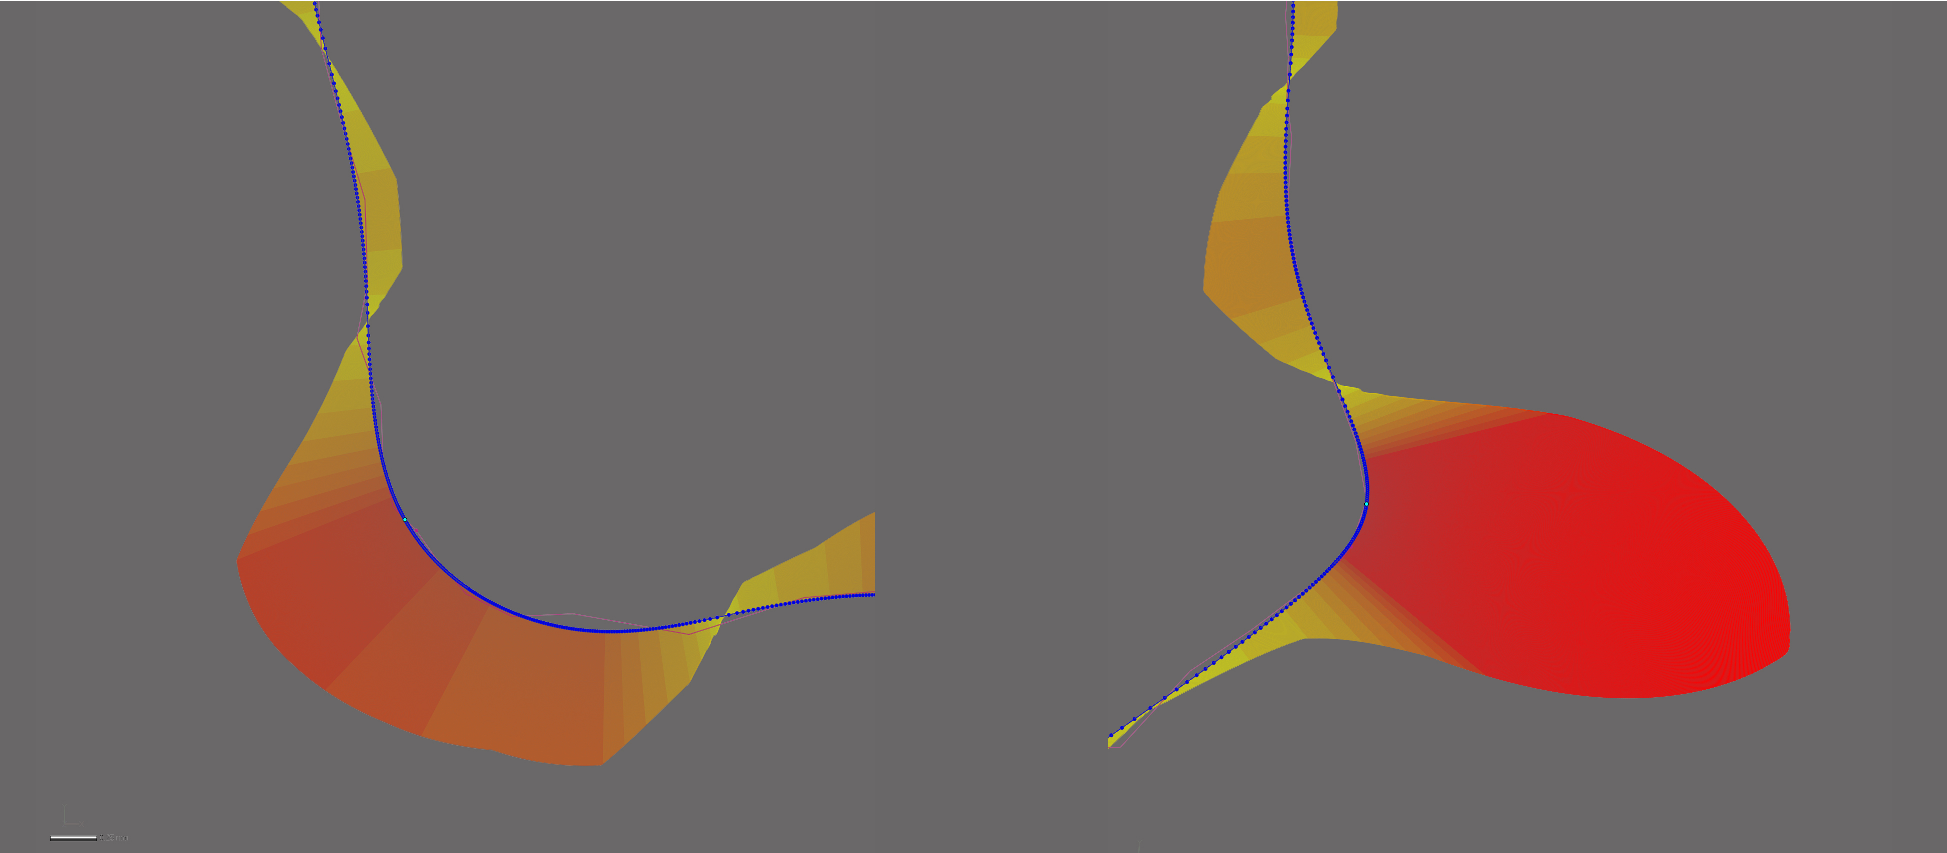
\includegraphics[width=\linewidth]{analysis/images/splinesplit1.pdf}
\caption{Horizontal tangent calculated, followed by insertion of reference point and reference plane (left). Reference plane used to cut spline at location of the horizontal tangent (right).}
\label{fig:figLM1}
\end{figure}

\begin{figure}[ht]\centering
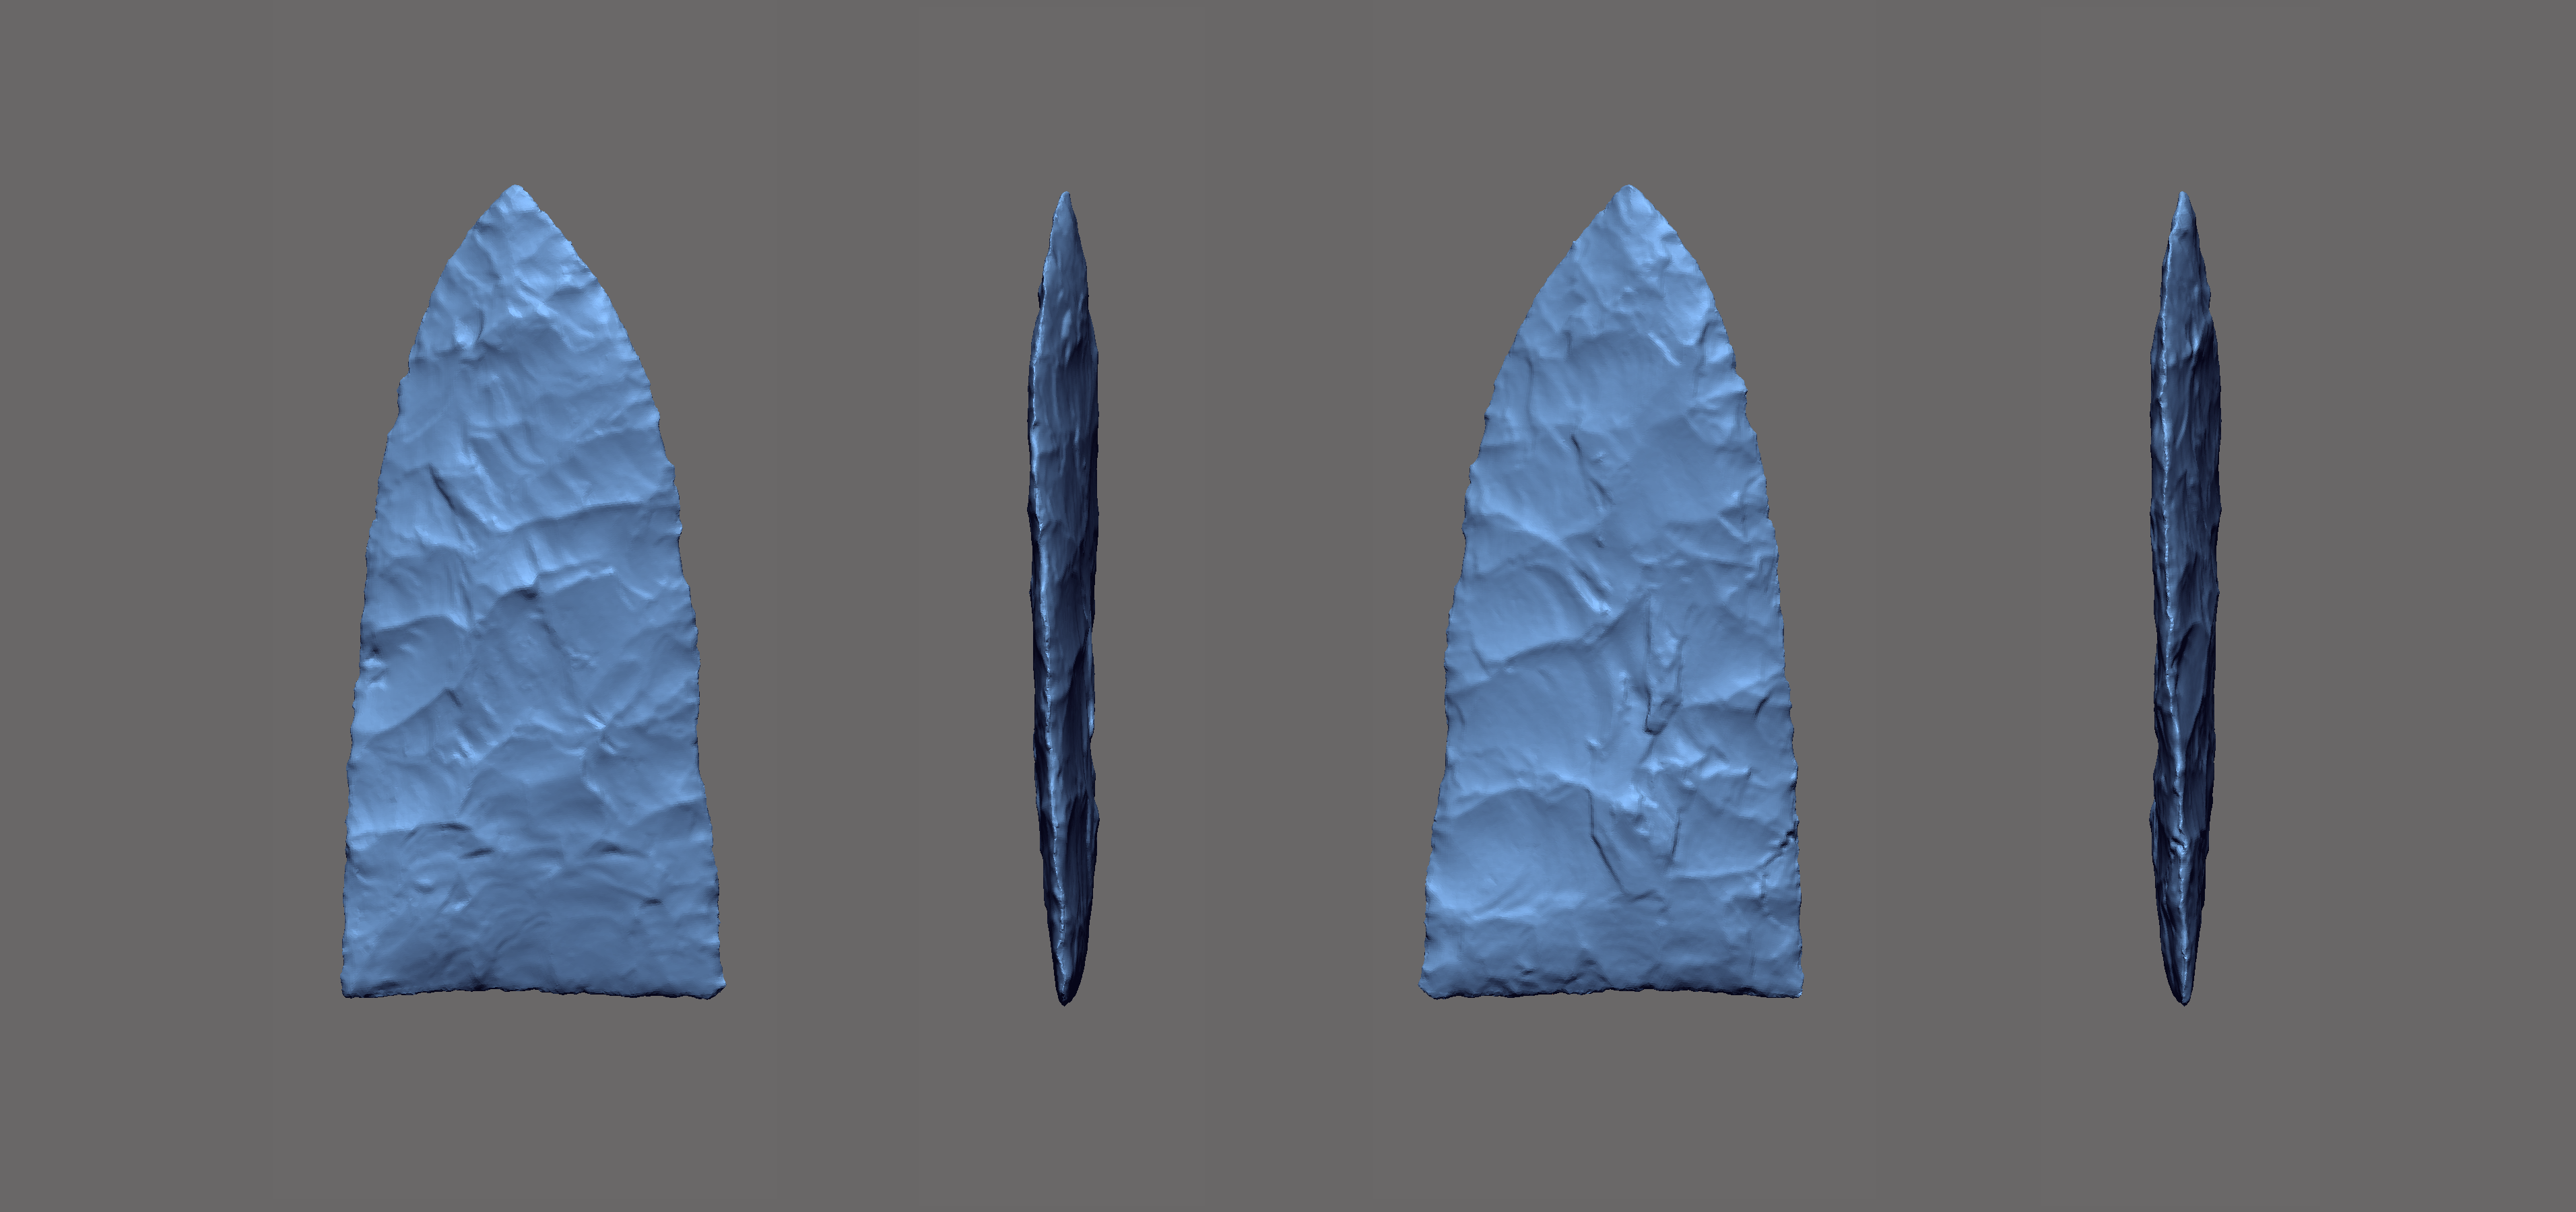
\includegraphics[width=\linewidth]{figbev}
\caption{Landmark and semilandmark placement. Note the axial twisting associated with beveling when the biface is aligned to the plane that intersects the first three landmarks.}
\label{fig:fig5}
\end{figure}

\subsection*{Analysis}

Landmark data were aligned to a global coordinate system \citep{RN11622,RN11623,RN11563}, achieved through generalised Procrustes superimposition \citep{RN478} performed in R 3.6.1 \citep{R} using the \textit{geomorph} library v.3.1.2 \citep{RN11530,RN1774}. Procrustes superimposition translates, scales, and rotates the coordinate data to allow for comparisons among objects \citep{RN11564,RN478}. The \textit{geomorph} package uses a partial Procrustes superimposition that projects the aligned specimens into tangent space subsequent to alignment in preparation for the use of multivariate methods that assume linear space \citep{RN1646,RN11563}.

Principal components analysis \citep{RN1746} was used to visualise shape variation among the bifaces. The shape changes described by each principal axis are commonly visualised using thin-plate spline warping of a reference 3D mesh \citep{RN1731,RN479}. A residual randomisation permutation procedure (RRPP; n = 10,000 permutations) was used for all Procrustes ANOVAs \citep{RN1655,RN11775}, which has higher statistical power and a greater ability to identify patterns in the data should they be present \citep{RN1719}. To assess whether shape changes with size (allometry), and differs by group (region), Procrustes ANOVAs \citep{RN1749} were also run that enlist effect-sizes (z-scores) computed as standard deviates of the generated sampling distributions \citep{RN1756}. 

\section*{Results}

The mean consensus configuration and Procrustes residuals were calculated by means of a generalised Procrustes analysis (GPA) \citep[Figure 3]{RN1720} (Figure ~\ref{fig:FigGPA}). This initial view of the dataset demonstrates the degree of variation that occurs at each site and in the combined sample. As an exploratory measure, GM methods---to include GPA---aid in clarifying shape differences associated with each population and in the production of novel \textit{a posteriori} hypotheses \citep{RN1720}. Further information and detail related to the analytical outputs can be found in \citep{RN20850}.

\begin{figure}[ht]\centering
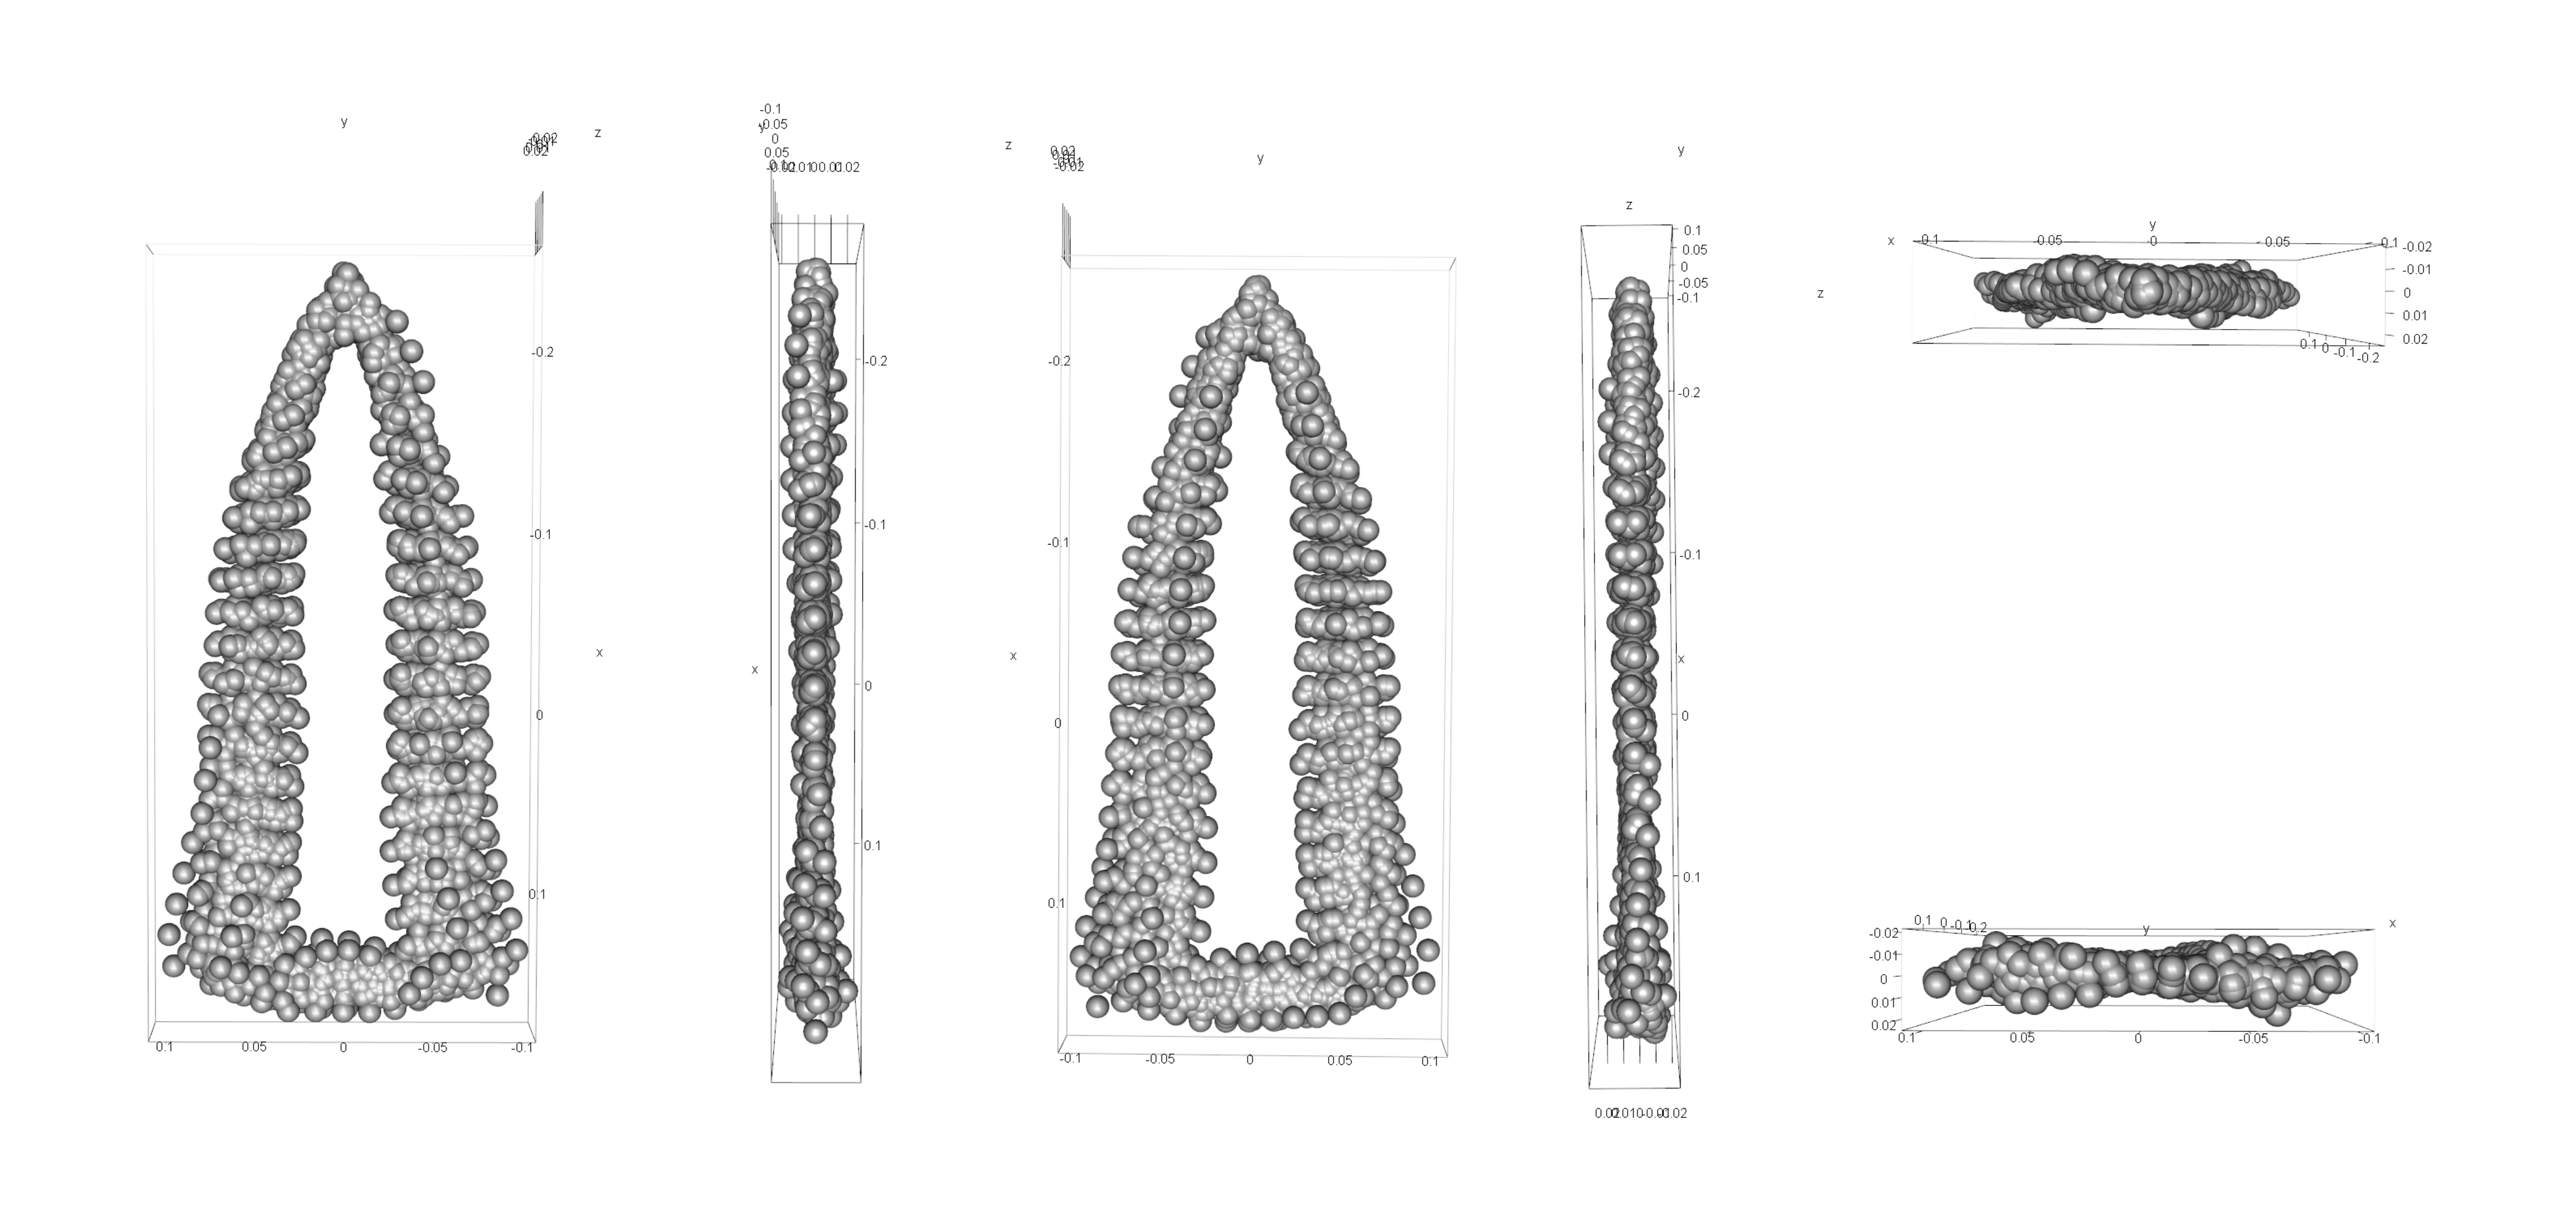
\includegraphics[width=\linewidth]{gpa3d}
\caption{Results of generalised Procrustes analysis.}
\label{fig:FigGPA}
\end{figure}

The mean consensus configuration for the sample from each region points toward a potentially significant difference in Gahagan biface morphology between the southern Caddo area and central Texas. The bifaces from Gahagan Mound generally include less recurve in the blade, and a base that is more convex than that of the bifaces from George C. Davis, where the mean consensus configuration of the base is slightly concave.

Principal components analysis (PCA) was conducted on scaled, translated, and rotated landmarks, and demonstrates that the first two PCs account for 62.46 (PC1) and 14.48 (PC2) percent of the variation in Gahagan biface shape (Figure ~\ref{fig:FigPCA}) \citep{RN20850}. Together, PC1 and PC2 account for over 77 percent of shape variation for Gahagan bifaces, with each remaining PC representing less than six percent of the variation \citep{RN20850}. The first two PCs are plotted in Figure ~\ref{fig:FigPCA}, where warp grids represent the shape changes along PC1 and PC2. This plot indicates that shape changes associated with PC1 articulate most readily with blades that range from broader at the minimum to narrow at the maximum, and base shapes that range from more concave at the minimum to flat or slightly convex at the maximum. Those shape changes associated with PC2 are dominated by differences in base shapes that range from narrow at minimum to broad at maximum, and blade shapes that are broader at minimum to narrower at maximum.

\begin{figure}[ht]\centering
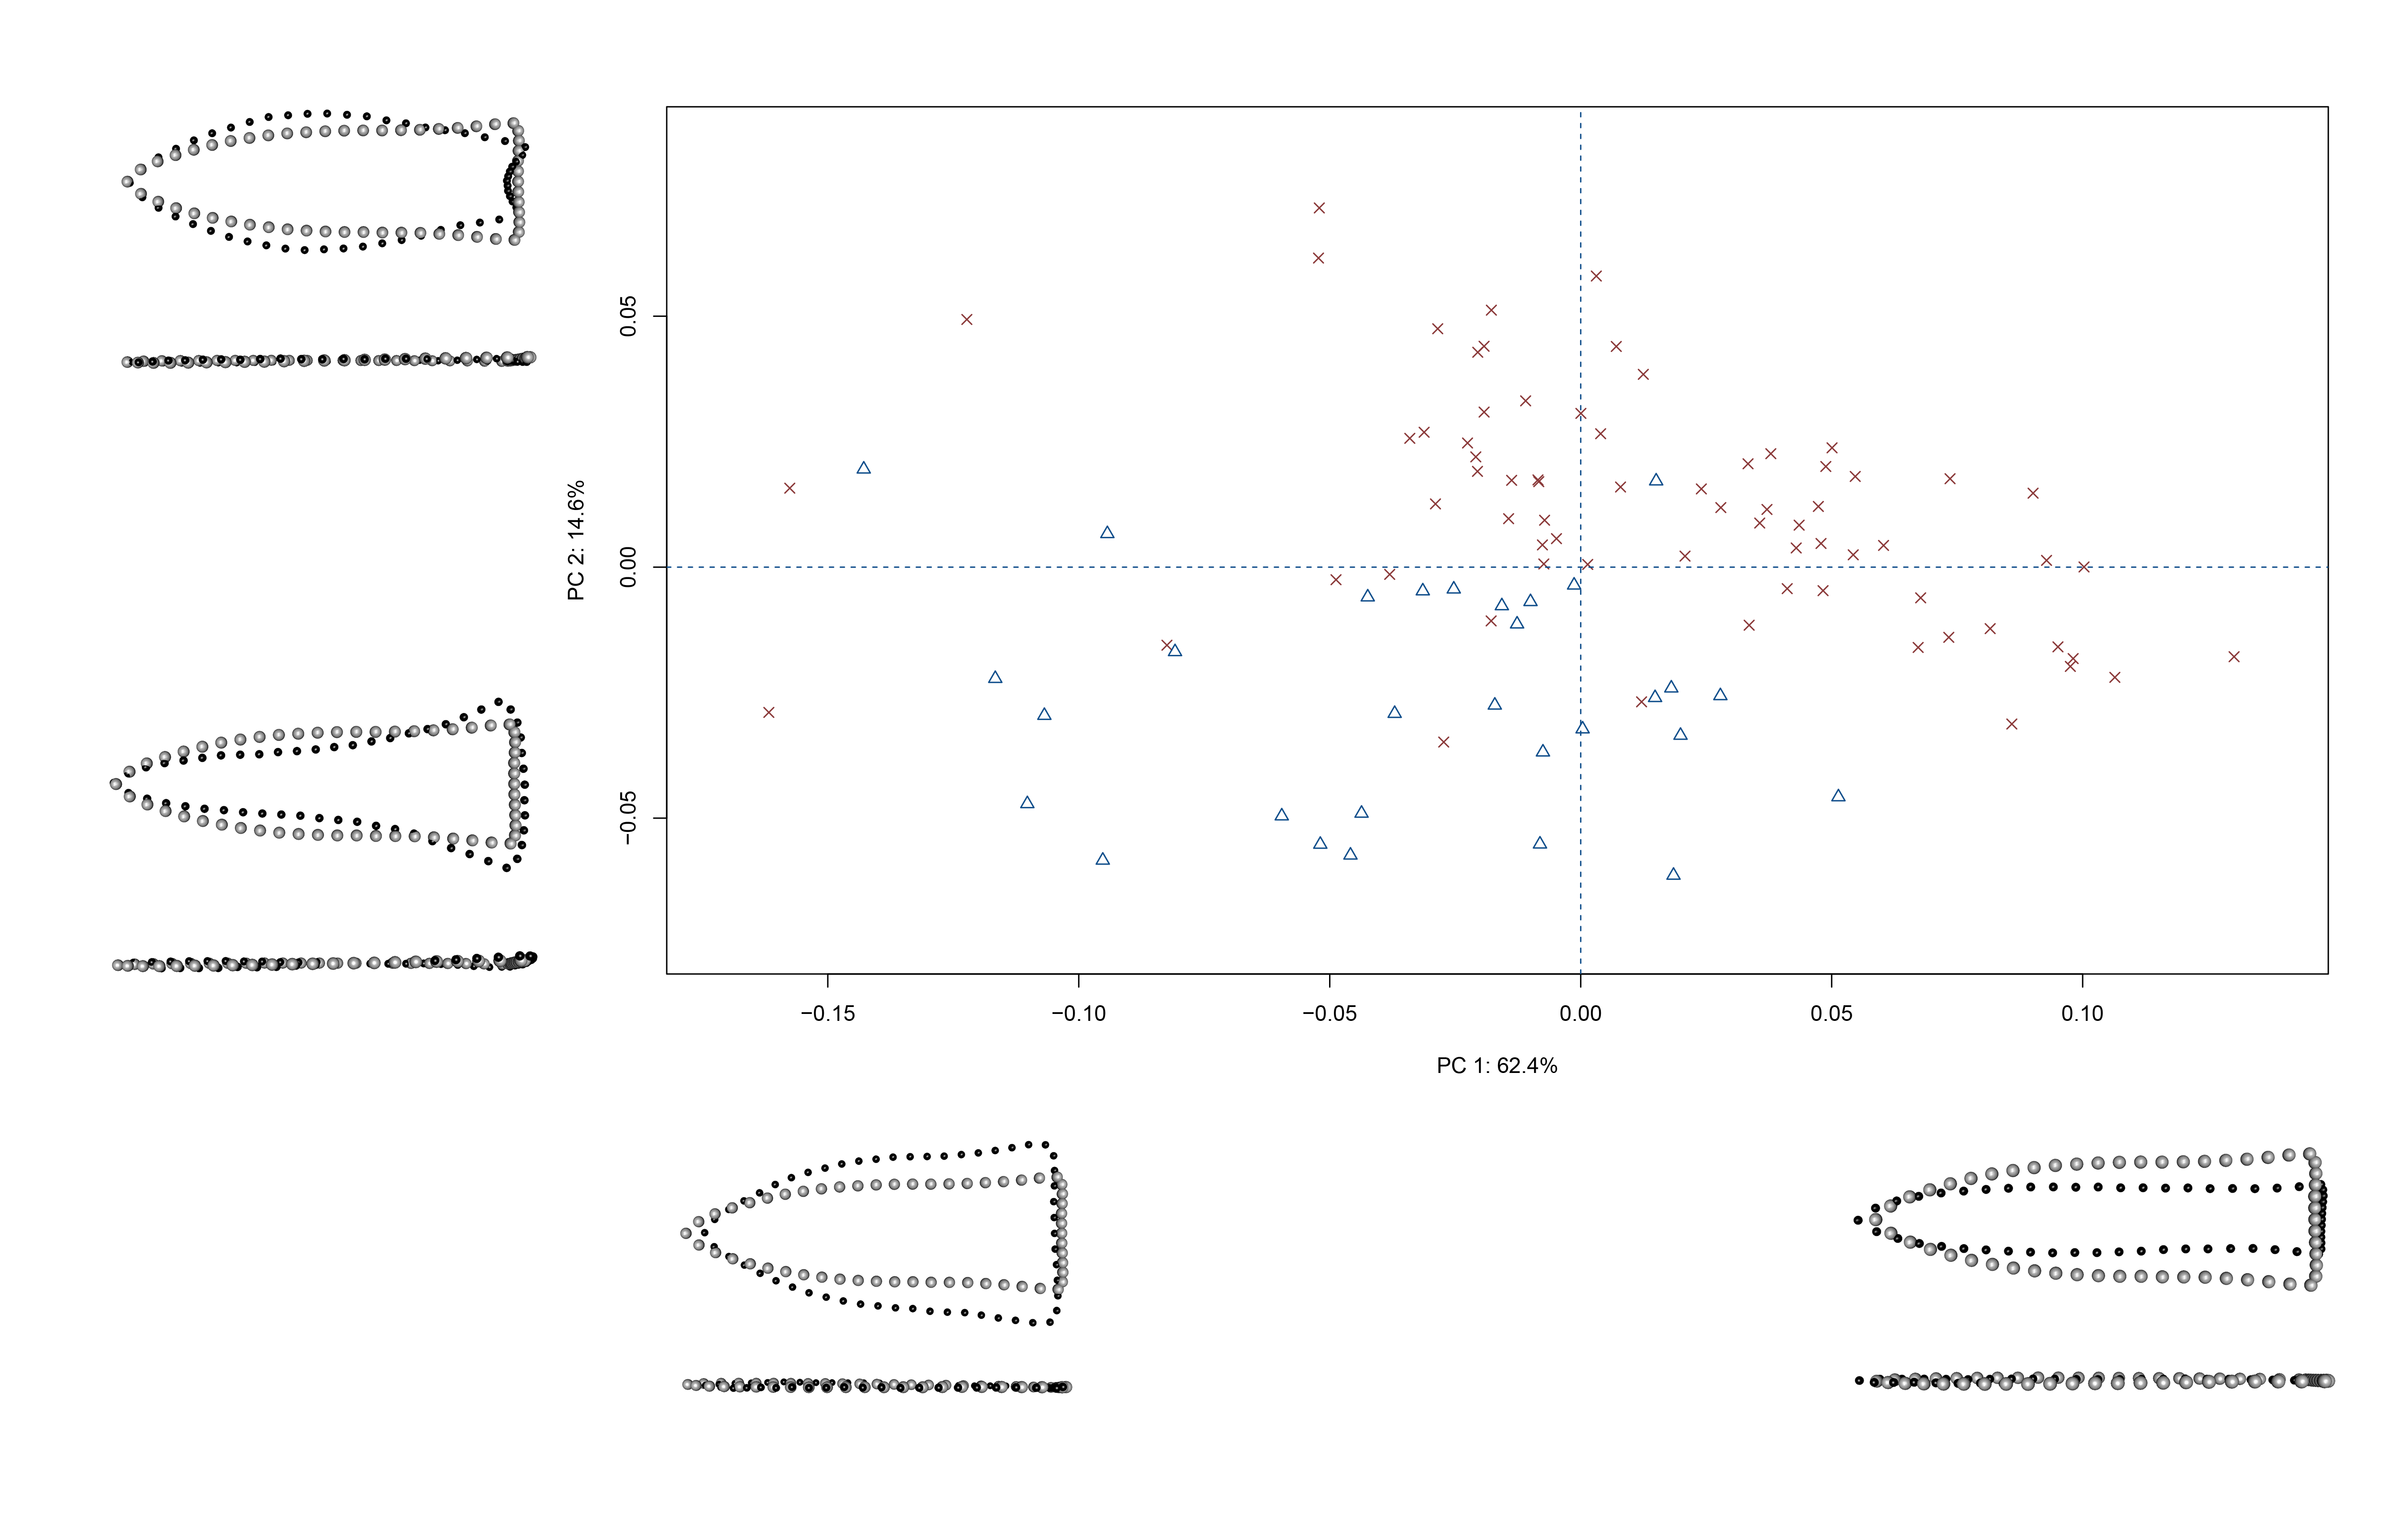
\includegraphics[width=\linewidth]{pca-warp-ref.pdf}
\caption{Principal components analysis plot (PC1/PC2) for Gahagan bifaces by region, where blue triangles represent bifaces from central Texas, and red X's represent those from the southern Caddo area. Reference shapes include the consensus configuration in gray, and the extremes of PC1 and PC2 in black.}
\label{fig:FigPCA}
\end{figure}

\section*{Discussion}



\subsection*{A theoretical discrepancy related to biface size}

(Figure ~\ref{fig:FigBox-CSize})

\begin{figure}[ht]\centering
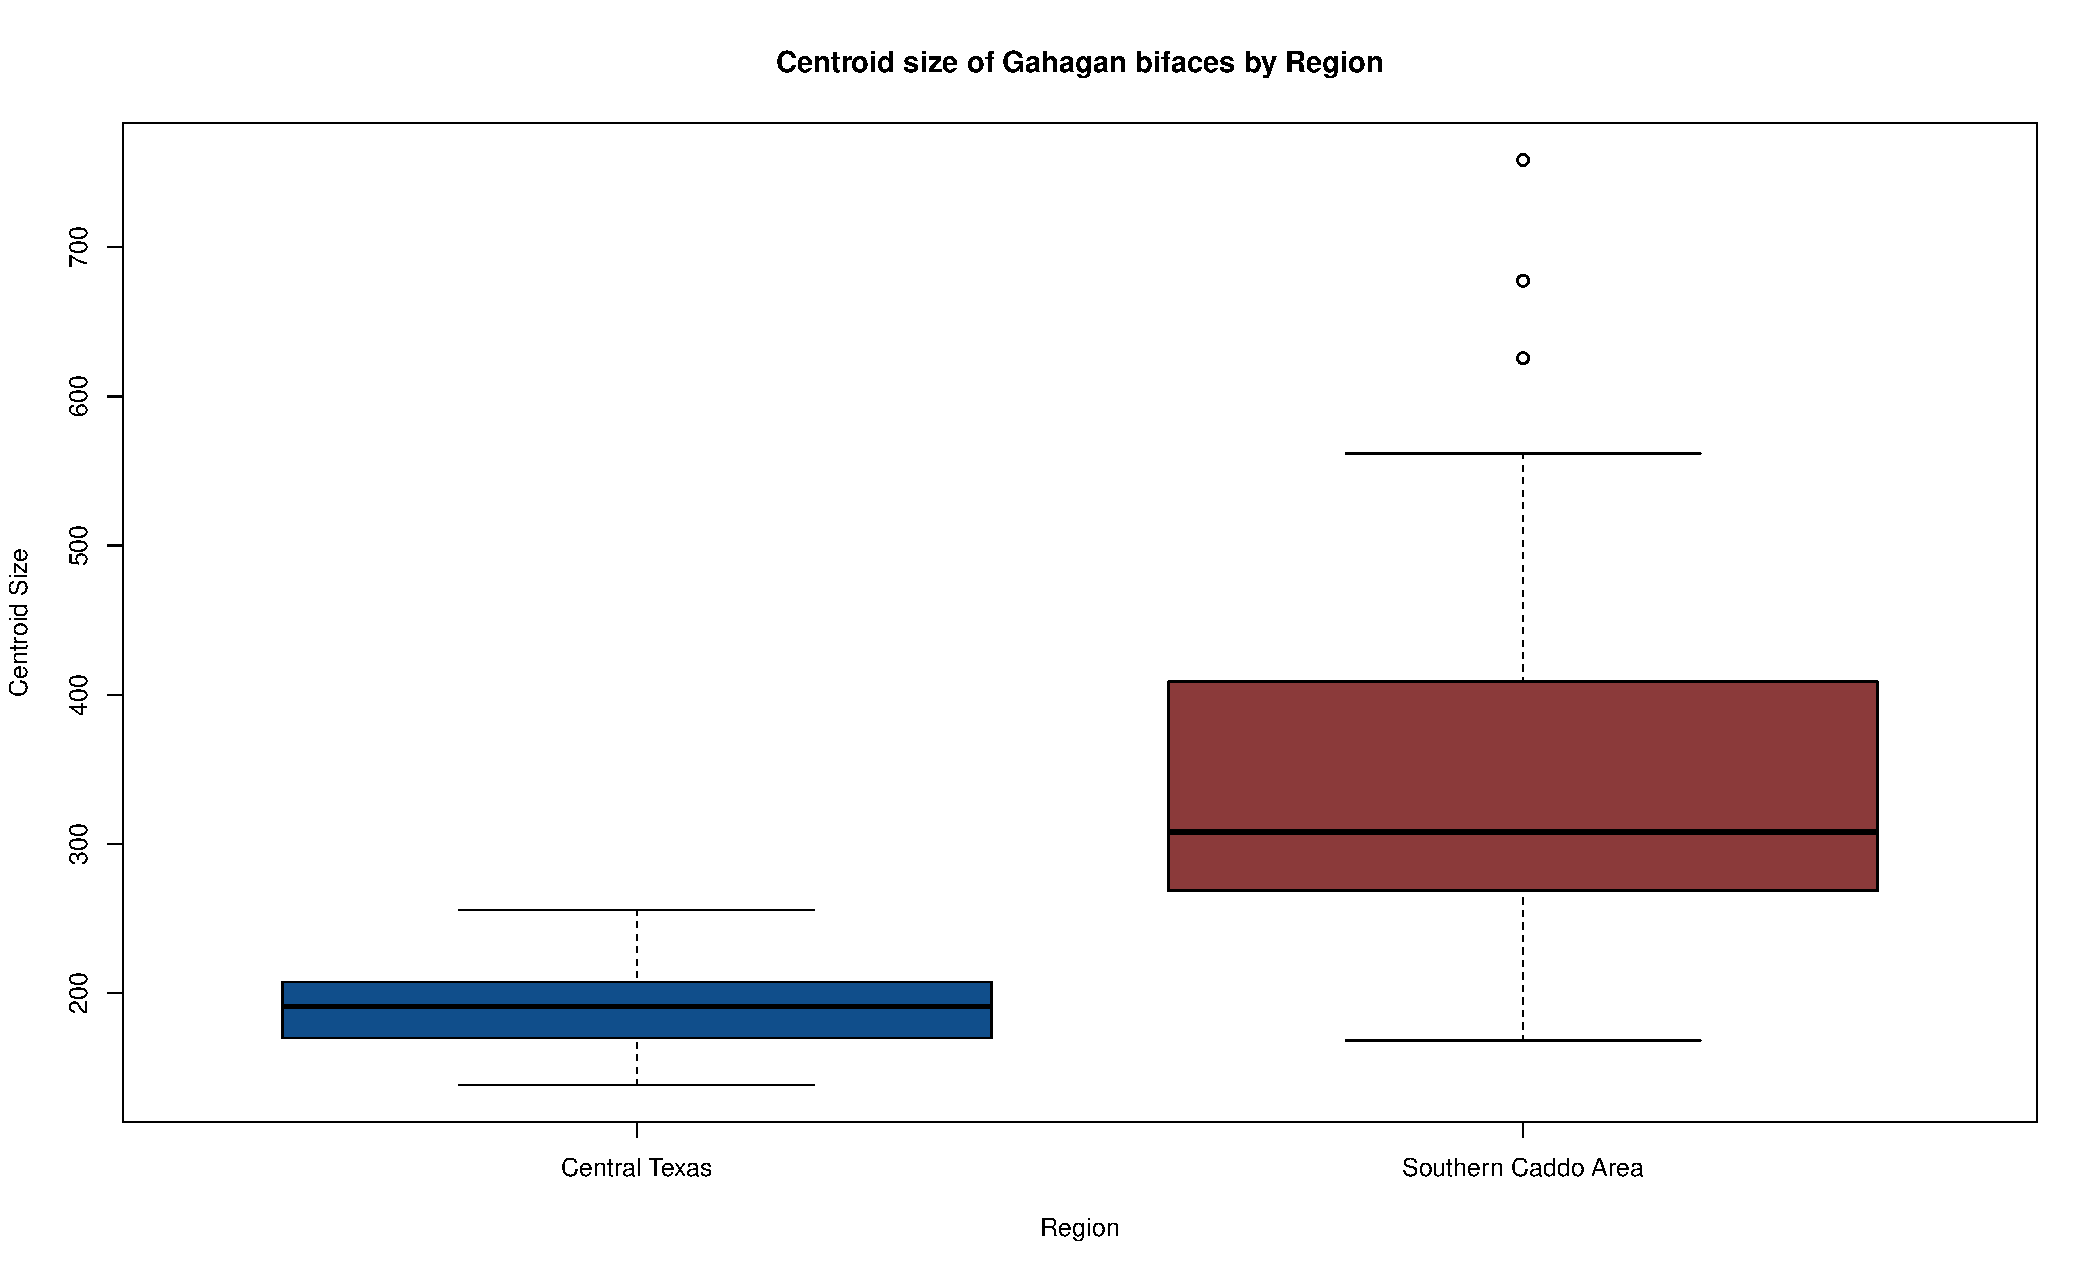
\includegraphics[width=\linewidth]{box-csize.pdf}
\caption{Boxplot of centroid size for Gahagan bifaces from central Texas (left), and the southern Caddo area (right).}
\label{fig:FigBox-CSize}
\end{figure}

\subsection*{Hunter-gatherers or Prairie Caddo?}



\subsection*{Future directions}

There are substantive challenges associated with the interpretation of Gahagan biface morphology. \citet{RN3684} notes that the makers of Gahagan bifaces likely resided at or near a location with ample raw materials. The working theory that Gahagan bifaces were not a product of Caddo manufacture is further evidenced by the absence of production failures at Caddo sites, and the absence of similar, locally-sourced raw materials. In a comparison of lithic reduction strategies, \citet{RN20701} compared the debitage sample from the western excavations at the George C. Davis site with that of 41MQ4, an Archaic (preceramic) site located around 100 km south of the Davis site, where raw material quality likely posed similar limitations on makers. Results indicated that the reduction strategy employed by the Caddo at George C. Davis was distinct from that of the Archaic sample \citep{RN20701}. That the Caddo are thought to have employed a distinct lithic reduction strategy is key to the interpretation of Caddo stone tools, which may be further evidenced through retouch or refurbishment of Gahagan bifaces. However, discriminating between patterns of Gahagan biface flake scars and debitage manufactured by central Texas knappers \citep{RN11568} and those made later by the Caddo is a substantive challenge that has not been addressed.

While true that many biface types may not warrant the time and labour investment associated with 3D data collection and analysis, 3D is necessary for the study of Gahagan bifaces. Morphological attributes associated with axial twisting and beveling hold substantive analytical value beyond the current study, and those data will be employed in a variety of ballistic simulations akin to the efforts of \citet{RN20857}. Due to the amount of axial twisting and beveling across the sample, other geometric morphometric approaches---like those aimed at discriminating among flaking patterns using EFA  \citep{RN253,RN4143,RN11975}---do not work for Gahagan bifaces. As a means of expanding upon these efforts, the next iteration of the analysis will include landmarks that articulate with a series of longitudinal cross-sections placed between the semilandmarks along the lateral edges (Figure ~\ref{fig:beveling}, left).

\begin{figure}[ht]\centering
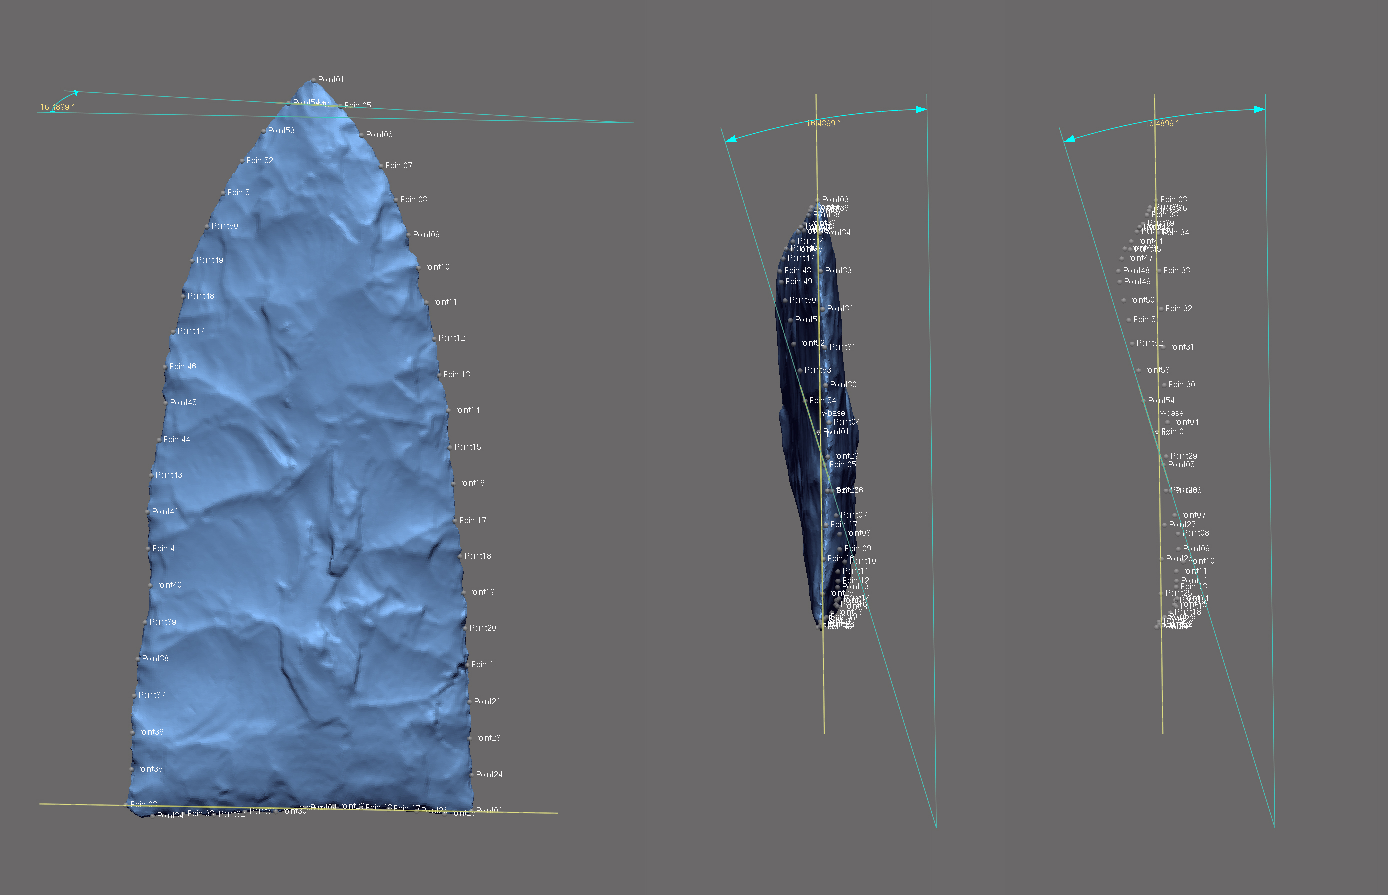
\includegraphics[width=\linewidth]{gahagan-beveling.pdf}
\caption{Degree of axial twisting calculated between two vectors placed between landmarks 2 and 3, and semilandmarks 5 and 54.}
\label{fig:beveling}
\end{figure}

Although not a component of the current analysis, attributes associated with retouch may articulate with beveling. Previously published methods of codifying and analysing retouch \citep{RN4308,RN3854} are being integrated into this analytical program, and another measure is under active development. Further work is needed to refine the latter approach; however, the measure is introduced here as it may hold value for studies that are currently planned or underway.

Enlisting the reference geometry used in the development of the current landmark configuration, the measure is comprised of an angle that occurs between two linear vectors. To calculate the angle from the aligned mesh, one vector is placed between landmarks 2 and 3 (base), then another between semilandmarks 5 and 54 (immediately below the tip) (Figure ~\ref{fig:beveling}, right), after which the angle between the two vectors can be calculated. It is not known whether this measure will correlate with those associated with retouch. However, should this angle be found to correlate with attributes related to size, spin torque, or other useful measures, it could hold value in future analyses.

\section*{Conclusion}


\section*{Data Accessibility Statement}

Data and code associated with this analysis can be accessed through the GitHub repository (\href{https://github.com/aksel-blaise/gahaganmorph2}{https://github.com/aksel-blaise/gahaganmorph2}), which is digitally curated on the Open Science Framework (OSF) (\href{https://osf.io/2g95w/}{DOI: 10.17605/OSF.IO/2G95W}). All 3D scan data (unprocessed and processed) are embargoed for a period of five years from the date of the last manuscript submission that employs them. The unprocessed 3D scan data were uploaded to the OSF, where the preprint of this paper and all supplementary materials are made available \citep{RN20850}.

\section*{Acknowledgments}

We extend our gratitude to the Caddo Tribe of Oklahoma, the Williamson Museum at Northwestern State University, the Louisiana State Exhibit Museum, the Texas Archeological Research Laboratory at The University of Texas at Austin, the Brazos Valley Museum of Natural History, the Texas Parks and Wildlife Department, and the Sam Noble Oklahoma Museum of Natural Science for the requisite permissions and access needed to generate the scans of Gahagan bifaces. Thanks to Harry J. Shafer, Jeffrey S. Girard, Hiram F. (Pete) Gregory, Julian A. Sitters, Timothy K. Perttula, and David K. Thulman for their comments on a draft of this manuscript. Thanks also to Dean C. Adams, Michael L. Collyer, Emma Sherratt, Lauren Butaric, and Kersten Bergstrom for their constructive criticisms, comments, and suggestions throughout the development of this research program, and to the editors and anonymous reviewers for their comments and constructive criticisms, which further improved the manuscript.

Components of this analytical work flow were developed and funded by a Preservation Technology and Training grant (P14AP00138) to RZS from the National Center for Preservation Technology and Training, and funding to scan the Gahagan bifaces at the Williamson Museum at Northwestern State University, Louisiana State Exhibit Museum, and Texas Archeological Research Laboratory at The University of Texas at Austin was provided to RZS by the Heritage Research Center at Stephen F. Austin State University.

\bibliography{mybibfile}

\end{document}
